% Options for packages loaded elsewhere
\PassOptionsToPackage{unicode}{hyperref}
\PassOptionsToPackage{hyphens}{url}
%
\documentclass[
  6pt,
]{article}
\usepackage{amsmath,amssymb}
\usepackage{iftex}
\ifPDFTeX
  \usepackage[T1]{fontenc}
  \usepackage[utf8]{inputenc}
  \usepackage{textcomp} % provide euro and other symbols
\else % if luatex or xetex
  \usepackage{unicode-math} % this also loads fontspec
  \defaultfontfeatures{Scale=MatchLowercase}
  \defaultfontfeatures[\rmfamily]{Ligatures=TeX,Scale=1}
\fi
\usepackage{lmodern}
\ifPDFTeX\else
  % xetex/luatex font selection
\fi
% Use upquote if available, for straight quotes in verbatim environments
\IfFileExists{upquote.sty}{\usepackage{upquote}}{}
\IfFileExists{microtype.sty}{% use microtype if available
  \usepackage[]{microtype}
  \UseMicrotypeSet[protrusion]{basicmath} % disable protrusion for tt fonts
}{}
\makeatletter
\@ifundefined{KOMAClassName}{% if non-KOMA class
  \IfFileExists{parskip.sty}{%
    \usepackage{parskip}
  }{% else
    \setlength{\parindent}{0pt}
    \setlength{\parskip}{6pt plus 2pt minus 1pt}}
}{% if KOMA class
  \KOMAoptions{parskip=half}}
\makeatother
\usepackage{xcolor}
\usepackage[top=2cm,bottom=2cm,right=2.5cm,left=2.5cm]{geometry}
\usepackage{color}
\usepackage{fancyvrb}
\newcommand{\VerbBar}{|}
\newcommand{\VERB}{\Verb[commandchars=\\\{\}]}
\DefineVerbatimEnvironment{Highlighting}{Verbatim}{commandchars=\\\{\}}
% Add ',fontsize=\small' for more characters per line
\usepackage{framed}
\definecolor{shadecolor}{RGB}{248,248,248}
\newenvironment{Shaded}{\begin{snugshade}}{\end{snugshade}}
\newcommand{\AlertTok}[1]{\textcolor[rgb]{0.94,0.16,0.16}{#1}}
\newcommand{\AnnotationTok}[1]{\textcolor[rgb]{0.56,0.35,0.01}{\textbf{\textit{#1}}}}
\newcommand{\AttributeTok}[1]{\textcolor[rgb]{0.13,0.29,0.53}{#1}}
\newcommand{\BaseNTok}[1]{\textcolor[rgb]{0.00,0.00,0.81}{#1}}
\newcommand{\BuiltInTok}[1]{#1}
\newcommand{\CharTok}[1]{\textcolor[rgb]{0.31,0.60,0.02}{#1}}
\newcommand{\CommentTok}[1]{\textcolor[rgb]{0.56,0.35,0.01}{\textit{#1}}}
\newcommand{\CommentVarTok}[1]{\textcolor[rgb]{0.56,0.35,0.01}{\textbf{\textit{#1}}}}
\newcommand{\ConstantTok}[1]{\textcolor[rgb]{0.56,0.35,0.01}{#1}}
\newcommand{\ControlFlowTok}[1]{\textcolor[rgb]{0.13,0.29,0.53}{\textbf{#1}}}
\newcommand{\DataTypeTok}[1]{\textcolor[rgb]{0.13,0.29,0.53}{#1}}
\newcommand{\DecValTok}[1]{\textcolor[rgb]{0.00,0.00,0.81}{#1}}
\newcommand{\DocumentationTok}[1]{\textcolor[rgb]{0.56,0.35,0.01}{\textbf{\textit{#1}}}}
\newcommand{\ErrorTok}[1]{\textcolor[rgb]{0.64,0.00,0.00}{\textbf{#1}}}
\newcommand{\ExtensionTok}[1]{#1}
\newcommand{\FloatTok}[1]{\textcolor[rgb]{0.00,0.00,0.81}{#1}}
\newcommand{\FunctionTok}[1]{\textcolor[rgb]{0.13,0.29,0.53}{\textbf{#1}}}
\newcommand{\ImportTok}[1]{#1}
\newcommand{\InformationTok}[1]{\textcolor[rgb]{0.56,0.35,0.01}{\textbf{\textit{#1}}}}
\newcommand{\KeywordTok}[1]{\textcolor[rgb]{0.13,0.29,0.53}{\textbf{#1}}}
\newcommand{\NormalTok}[1]{#1}
\newcommand{\OperatorTok}[1]{\textcolor[rgb]{0.81,0.36,0.00}{\textbf{#1}}}
\newcommand{\OtherTok}[1]{\textcolor[rgb]{0.56,0.35,0.01}{#1}}
\newcommand{\PreprocessorTok}[1]{\textcolor[rgb]{0.56,0.35,0.01}{\textit{#1}}}
\newcommand{\RegionMarkerTok}[1]{#1}
\newcommand{\SpecialCharTok}[1]{\textcolor[rgb]{0.81,0.36,0.00}{\textbf{#1}}}
\newcommand{\SpecialStringTok}[1]{\textcolor[rgb]{0.31,0.60,0.02}{#1}}
\newcommand{\StringTok}[1]{\textcolor[rgb]{0.31,0.60,0.02}{#1}}
\newcommand{\VariableTok}[1]{\textcolor[rgb]{0.00,0.00,0.00}{#1}}
\newcommand{\VerbatimStringTok}[1]{\textcolor[rgb]{0.31,0.60,0.02}{#1}}
\newcommand{\WarningTok}[1]{\textcolor[rgb]{0.56,0.35,0.01}{\textbf{\textit{#1}}}}
\usepackage{longtable,booktabs,array}
\usepackage{calc} % for calculating minipage widths
% Correct order of tables after \paragraph or \subparagraph
\usepackage{etoolbox}
\makeatletter
\patchcmd\longtable{\par}{\if@noskipsec\mbox{}\fi\par}{}{}
\makeatother
% Allow footnotes in longtable head/foot
\IfFileExists{footnotehyper.sty}{\usepackage{footnotehyper}}{\usepackage{footnote}}
\makesavenoteenv{longtable}
\usepackage{graphicx}
\makeatletter
\def\maxwidth{\ifdim\Gin@nat@width>\linewidth\linewidth\else\Gin@nat@width\fi}
\def\maxheight{\ifdim\Gin@nat@height>\textheight\textheight\else\Gin@nat@height\fi}
\makeatother
% Scale images if necessary, so that they will not overflow the page
% margins by default, and it is still possible to overwrite the defaults
% using explicit options in \includegraphics[width, height, ...]{}
\setkeys{Gin}{width=\maxwidth,height=\maxheight,keepaspectratio}
% Set default figure placement to htbp
\makeatletter
\def\fps@figure{htbp}
\makeatother
\setlength{\emergencystretch}{3em} % prevent overfull lines
\providecommand{\tightlist}{%
  \setlength{\itemsep}{0pt}\setlength{\parskip}{0pt}}
\setcounter{secnumdepth}{5}
\ifLuaTeX
\usepackage[bidi=basic]{babel}
\else
\usepackage[bidi=default]{babel}
\fi
\babelprovide[main,import]{french}
% get rid of language-specific shorthands (see #6817):
\let\LanguageShortHands\languageshorthands
\def\languageshorthands#1{}
\usepackage{fvextra}
\DefineVerbatimEnvironment{Highlighting}{Verbatim}{breaklines,commandchars=\\\{\}}
\RecustomVerbatimEnvironment{verbatim}{Verbatim}{breaklines,commandchars=\\\{\}}
\renewcommand{\baselinestretch}{1.1}
\usepackage{booktabs}
\usepackage{longtable}
\usepackage{array}
\usepackage{multirow}
\usepackage{wrapfig}
\usepackage{float}
\usepackage{colortbl}
\usepackage{pdflscape}
\usepackage{tabu}
\usepackage{threeparttable}
\usepackage{threeparttablex}
\usepackage[normalem]{ulem}
\usepackage{makecell}
\usepackage{xcolor}
\ifLuaTeX
  \usepackage{selnolig}  % disable illegal ligatures
\fi
\usepackage{bookmark}
\IfFileExists{xurl.sty}{\usepackage{xurl}}{} % add URL line breaks if available
\urlstyle{same}
\hypersetup{
  pdftitle={Projet en atelier statistique avec R},
  pdfauthor={Yassine Hammi},
  pdflang={fr},
  hidelinks,
  pdfcreator={LaTeX via pandoc}}

\title{Projet en atelier statistique avec R}
\usepackage{etoolbox}
\makeatletter
\providecommand{\subtitle}[1]{% add subtitle to \maketitle
  \apptocmd{\@title}{\par {\large #1 \par}}{}{}
}
\makeatother
\subtitle{Analyse de l Impact des Performances des Joueurs sur les
Résultats d equipe}
\author{Yassine Hammi}
\date{2024-11-26}

\begin{document}
\maketitle

{
\setcounter{tocdepth}{6}
\tableofcontents
}
\newpage

\section{Introduction}\label{introduction}

Dans le domaine sportif, la performance individuelle des joueurs peut
influencer directement ou indirectement les résultats globaux de leur
équipe. Cependant, comprendre précisément cette relation reste un défi.

Quels sont les facteurs clés individuelle qui influencent les
performances collectives ? Quels types de joueurs ont un rôle
déterminant sur les victoires ou les défaites? Cette analyse est
essentielle pour optimiser la gestion des équipes et améliorer leurs
performances.

Pour commencer, nous allons aborder la question d'exploration
fondamentale, qui sera le point de départ de notre analyse à travers les
différentes étapes. Nous permettant de spécifier les variables clés à
observer, de collecter des données exhaustives, de les prétraiter avec
rigueur, d'effectuer une analyse approfondie et enfin de présenter des
résultats interprétables.

\subsection{Question principale
d'exploration}\label{question-principale-dexploration}

Comment les performances individuelles des joueurs influencent-elles les
résultats et la performance globale de leur équipe ?

En examinant de près les principales raisons, nous espérons obtenir une
meilleure compréhension sur les perforamnces pour chaque joueur
individuelle et comme conséquences la performance d'equipe et comment
cela influence l'echec ou la reussite de l'equipe.

\subsection{Spécification des
Variables}\label{spuxe9cification-des-variables}

Pour mener à bien notre analyse, nous nous appuierons sur differents
sources de données cruciales telque ``Performance des joueurs
individuels'' et leur ``Resultats des matchs'', ``Performance
collective''

\section{Collecte de Données}\label{collecte-de-donnuxe9es}

Collection de données s'agit d'une étape cruciale pour l'ensemble du
projet, tant que nous disposons de données bien structurés, nous pouvons
effectuer une meilleure analyse plus approfondie.

il est important d'identifier notre sources de données

\subsection{Identification}\label{identification}

\begin{itemize}
\item
  Kaggle: as the world's largest data science community with powerful
  tools and resources to help us achieve our data science goals and
  objectifs.
\item
  Github : nous pouvons trouver plusieurs projets open source concernant
  le football, avec des données mises à jour sur les joueurs et les
  équipes.
\end{itemize}

\subsection{Importation}\label{importation}

Au début de notre analyse, nous commençons par intégrer les données
essentielles à partir des sources distincts.

\begin{Shaded}
\begin{Highlighting}[]
\CommentTok{\# Installation de package si n\textquotesingle{}existe pas }
\ControlFlowTok{if}\NormalTok{ (}\SpecialCharTok{!}\FunctionTok{require}\NormalTok{(readr) ) \{}\FunctionTok{install.packages}\NormalTok{(}\StringTok{"readr"}\NormalTok{ , }\AttributeTok{repos =} \StringTok{"http://cran.us.r{-}project.org"}\NormalTok{)\}}
\ControlFlowTok{if}\NormalTok{ (}\SpecialCharTok{!}\FunctionTok{require}\NormalTok{(dplyr) ) \{}\FunctionTok{install.packages}\NormalTok{(}\StringTok{"dplyr"}\NormalTok{ , }\AttributeTok{repos =} \StringTok{"http://cran.us.r{-}project.org"}\NormalTok{)\}}
\ControlFlowTok{if}\NormalTok{ (}\SpecialCharTok{!}\FunctionTok{require}\NormalTok{(tidyr) ) \{}\FunctionTok{install.packages}\NormalTok{(}\StringTok{"tidyr"}\NormalTok{ , }\AttributeTok{repos =} \StringTok{"http://cran.us.r{-}project.org"}\NormalTok{)\}}
\ControlFlowTok{if}\NormalTok{ (}\SpecialCharTok{!}\FunctionTok{require}\NormalTok{(ggplot2) ) \{}\FunctionTok{install.packages}\NormalTok{(}\StringTok{"ggplot2"}\NormalTok{ , }\AttributeTok{repos =} \StringTok{"http://cran.us.r{-}project.org"}\NormalTok{)\}}
\ControlFlowTok{if}\NormalTok{ (}\SpecialCharTok{!}\FunctionTok{require}\NormalTok{(ggcorrplot) ) \{}\FunctionTok{install.packages}\NormalTok{(}\StringTok{"ggcorrplot"}\NormalTok{ , }\AttributeTok{repos =} \StringTok{"http://cran.us.r{-}project.org"}\NormalTok{)\}}
\ControlFlowTok{if}\NormalTok{ (}\SpecialCharTok{!}\FunctionTok{require}\NormalTok{(fmsb) ) \{}\FunctionTok{install.packages}\NormalTok{(}\StringTok{"fmsb"}\NormalTok{ , }\AttributeTok{repos =} \StringTok{"http://cran.us.r{-}project.org"}\NormalTok{)\}}
\ControlFlowTok{if}\NormalTok{ (}\SpecialCharTok{!}\FunctionTok{require}\NormalTok{(ggradar) ) \{}\FunctionTok{install.packages}\NormalTok{(}\StringTok{"ggradar"}\NormalTok{ , }\AttributeTok{repos =} \StringTok{"http://cran.us.r{-}project.org"}\NormalTok{)\}}
\ControlFlowTok{if}\NormalTok{ (}\SpecialCharTok{!}\FunctionTok{require}\NormalTok{(reshape2) ) \{}\FunctionTok{install.packages}\NormalTok{(}\StringTok{"reshape2"}\NormalTok{ , }\AttributeTok{repos =} \StringTok{"http://cran.us.r{-}project.org"}\NormalTok{)\}}
\ControlFlowTok{if}\NormalTok{ (}\SpecialCharTok{!}\FunctionTok{require}\NormalTok{(coefplot) ) \{}\FunctionTok{install.packages}\NormalTok{(}\StringTok{"coefplot"}\NormalTok{ , }\AttributeTok{repos =} \StringTok{"http://cran.us.r{-}project.org"}\NormalTok{)\}}

\CommentTok{\# Chargement de package }
\FunctionTok{library}\NormalTok{(readr)}
\FunctionTok{library}\NormalTok{(knitr)}
\FunctionTok{library}\NormalTok{(ggplot2)}
\FunctionTok{library}\NormalTok{(reshape2)}
\FunctionTok{library}\NormalTok{(corrplot)}
\FunctionTok{library}\NormalTok{(coefplot)}


\CommentTok{\# Importation de donneés depuis fichier excel }
\CommentTok{\# Cette fichier est importé depuis kaggle}
\CommentTok{\# Comporte les donneés de championnat d\textquotesingle{}Espagne de football de première division}

\NormalTok{LaLigaPlayers }\OtherTok{\textless{}{-}} \FunctionTok{read\_csv}\NormalTok{(}\StringTok{"C:/Users/21655/Desktop/Projet\_DS\_Yassine/Data/S2324{-}laliga{-}players.csv"}\NormalTok{)}
\CommentTok{\# Dimension de notre dataset }
\FunctionTok{dim}\NormalTok{(LaLigaPlayers) }\CommentTok{\# 3615 lignes , 150 columns }
\CommentTok{\# Affichage de dooneés }
\FunctionTok{kable}\NormalTok{(}\FunctionTok{head}\NormalTok{(LaLigaPlayers[,}\DecValTok{7}\SpecialCharTok{:}\DecValTok{13}\NormalTok{],}\DecValTok{6}\NormalTok{),}\AttributeTok{caption =} \StringTok{"LaLiga {-} sample 6 lignes avec 7 columns"}\NormalTok{)}
\end{Highlighting}
\end{Shaded}

\begin{verbatim}
## [1] 3615  150
\end{verbatim}

\begin{longtable}[]{@{}
  >{\raggedright\arraybackslash}p{(\columnwidth - 12\tabcolsep) * \real{0.1408}}
  >{\raggedright\arraybackslash}p{(\columnwidth - 12\tabcolsep) * \real{0.1549}}
  >{\raggedright\arraybackslash}p{(\columnwidth - 12\tabcolsep) * \real{0.0986}}
  >{\raggedright\arraybackslash}p{(\columnwidth - 12\tabcolsep) * \real{0.1972}}
  >{\raggedright\arraybackslash}p{(\columnwidth - 12\tabcolsep) * \real{0.2113}}
  >{\raggedleft\arraybackslash}p{(\columnwidth - 12\tabcolsep) * \real{0.0986}}
  >{\raggedleft\arraybackslash}p{(\columnwidth - 12\tabcolsep) * \real{0.0986}}@{}}
\caption{LaLiga - sample 6 lignes avec 7 columns}\tabularnewline
\toprule\noalign{}
\begin{minipage}[b]{\linewidth}\raggedright
firstname
\end{minipage} & \begin{minipage}[b]{\linewidth}\raggedright
lastname
\end{minipage} & \begin{minipage}[b]{\linewidth}\raggedright
gender
\end{minipage} & \begin{minipage}[b]{\linewidth}\raggedright
date\_of\_birth
\end{minipage} & \begin{minipage}[b]{\linewidth}\raggedright
place\_of\_birth
\end{minipage} & \begin{minipage}[b]{\linewidth}\raggedleft
weight
\end{minipage} & \begin{minipage}[b]{\linewidth}\raggedleft
height
\end{minipage} \\
\midrule\noalign{}
\endfirsthead
\toprule\noalign{}
\begin{minipage}[b]{\linewidth}\raggedright
firstname
\end{minipage} & \begin{minipage}[b]{\linewidth}\raggedright
lastname
\end{minipage} & \begin{minipage}[b]{\linewidth}\raggedright
gender
\end{minipage} & \begin{minipage}[b]{\linewidth}\raggedright
date\_of\_birth
\end{minipage} & \begin{minipage}[b]{\linewidth}\raggedright
place\_of\_birth
\end{minipage} & \begin{minipage}[b]{\linewidth}\raggedleft
weight
\end{minipage} & \begin{minipage}[b]{\linewidth}\raggedleft
height
\end{minipage} \\
\midrule\noalign{}
\endhead
\bottomrule\noalign{}
\endlastfoot
Aarón & Escandell & male & 1995-09-27 & Carcagente & 71 & 185 \\
Abde & Ezzalzouli & male & 2001-12-17 & Beni Melal & 72 & 177 \\
Abde & Raihani & male & 2004-02-03 & Barcelona & NA & 187 \\
Abde & Rebbach & male & 1998-08-11 & Bilda & NA & 176 \\
Abdel & Abqar & male & 1999-03-10 & Settat & 80 & 188 \\
Abdul & Mumin & male & 1998-06-06 & Accra & 79 & 188 \\
\end{longtable}

\begin{Shaded}
\begin{Highlighting}[]
\CommentTok{\# Chargement de package pour extraire des données depuis l\textquotesingle{}internet }
\FunctionTok{library}\NormalTok{(rvest)}
 
\CommentTok{\# Le lien d’où allons extraire les informations d\textquotesingle{}une equipe}
\CommentTok{\# Dans ce cas nous avons choisis l\textquotesingle{}equipe "Real Madrid" }
\NormalTok{link }\OtherTok{\textless{}{-}}\StringTok{"https://fbref.com/fr/equipes/53a2f082/2023{-}2024/Statistiques{-}Real{-}Madrid"}

\NormalTok{page }\OtherTok{\textless{}{-}} \FunctionTok{read\_html}\NormalTok{(link,}\AttributeTok{header=}\ConstantTok{FALSE}\NormalTok{)}

\CommentTok{\# Nous avons extrait les tables dans cette page }
\NormalTok{tables }\OtherTok{\textless{}{-}}\NormalTok{ page }\SpecialCharTok{\%\textgreater{}\%}
  \FunctionTok{html\_nodes}\NormalTok{(}\StringTok{"table"}\NormalTok{) }\SpecialCharTok{\%\textgreater{}\%}
  \FunctionTok{html\_table}\NormalTok{(}\AttributeTok{fill =} \ConstantTok{TRUE}\NormalTok{)}

\CommentTok{\# Mettre le deuxième tableau dans notre dataset MatchesRM}
\ControlFlowTok{if}\NormalTok{(}\FunctionTok{length}\NormalTok{(tables)}\SpecialCharTok{\textgreater{}}\DecValTok{0}\NormalTok{)\{}
\NormalTok{  MatchesRM }\OtherTok{\textless{}{-}}\NormalTok{ tables[[}\DecValTok{2}\NormalTok{]]}
  \FunctionTok{dim}\NormalTok{(MatchesRM)  }\CommentTok{\# 55 lignes , 20 columns }
  \FunctionTok{kable}\NormalTok{(}\FunctionTok{head}\NormalTok{(MatchesRM[,}\DecValTok{4}\SpecialCharTok{:}\DecValTok{13}\NormalTok{],}\DecValTok{6}\NormalTok{),}\AttributeTok{caption=}\StringTok{"Matches{-}RM"}\NormalTok{) }
\NormalTok{\} }\ControlFlowTok{else}\NormalTok{ \{}
  \FunctionTok{print}\NormalTok{(}\StringTok{"aucun table trouveé"}\NormalTok{)}
\NormalTok{\}}
\end{Highlighting}
\end{Shaded}

\begin{longtable}[]{@{}
  >{\raggedright\arraybackslash}p{(\columnwidth - 18\tabcolsep) * \real{0.2133}}
  >{\raggedright\arraybackslash}p{(\columnwidth - 18\tabcolsep) * \real{0.0667}}
  >{\raggedright\arraybackslash}p{(\columnwidth - 18\tabcolsep) * \real{0.1333}}
  >{\raggedright\arraybackslash}p{(\columnwidth - 18\tabcolsep) * \real{0.1200}}
  >{\raggedright\arraybackslash}p{(\columnwidth - 18\tabcolsep) * \real{0.0400}}
  >{\raggedright\arraybackslash}p{(\columnwidth - 18\tabcolsep) * \real{0.0400}}
  >{\raggedright\arraybackslash}p{(\columnwidth - 18\tabcolsep) * \real{0.2133}}
  >{\raggedleft\arraybackslash}p{(\columnwidth - 18\tabcolsep) * \real{0.0533}}
  >{\raggedleft\arraybackslash}p{(\columnwidth - 18\tabcolsep) * \real{0.0533}}
  >{\raggedleft\arraybackslash}p{(\columnwidth - 18\tabcolsep) * \real{0.0667}}@{}}
\caption{Matches-RM}\tabularnewline
\toprule\noalign{}
\begin{minipage}[b]{\linewidth}\raggedright
Tour
\end{minipage} & \begin{minipage}[b]{\linewidth}\raggedright
Jour
\end{minipage} & \begin{minipage}[b]{\linewidth}\raggedright
Tribune
\end{minipage} & \begin{minipage}[b]{\linewidth}\raggedright
Résultat
\end{minipage} & \begin{minipage}[b]{\linewidth}\raggedright
BM
\end{minipage} & \begin{minipage}[b]{\linewidth}\raggedright
BE
\end{minipage} & \begin{minipage}[b]{\linewidth}\raggedright
Adversaire
\end{minipage} & \begin{minipage}[b]{\linewidth}\raggedleft
xG
\end{minipage} & \begin{minipage}[b]{\linewidth}\raggedleft
xGA
\end{minipage} & \begin{minipage}[b]{\linewidth}\raggedleft
Poss
\end{minipage} \\
\midrule\noalign{}
\endfirsthead
\toprule\noalign{}
\begin{minipage}[b]{\linewidth}\raggedright
Tour
\end{minipage} & \begin{minipage}[b]{\linewidth}\raggedright
Jour
\end{minipage} & \begin{minipage}[b]{\linewidth}\raggedright
Tribune
\end{minipage} & \begin{minipage}[b]{\linewidth}\raggedright
Résultat
\end{minipage} & \begin{minipage}[b]{\linewidth}\raggedright
BM
\end{minipage} & \begin{minipage}[b]{\linewidth}\raggedright
BE
\end{minipage} & \begin{minipage}[b]{\linewidth}\raggedright
Adversaire
\end{minipage} & \begin{minipage}[b]{\linewidth}\raggedleft
xG
\end{minipage} & \begin{minipage}[b]{\linewidth}\raggedleft
xGA
\end{minipage} & \begin{minipage}[b]{\linewidth}\raggedleft
Poss
\end{minipage} \\
\midrule\noalign{}
\endhead
\bottomrule\noalign{}
\endlastfoot
Journée 1 & Sam & Extérieur & V & 2 & 0 & Athletic Club & 0.9 & 0.4 &
54 \\
Journée 2 & Sam & Extérieur & V & 3 & 1 & Almería & 2.0 & 1.3 & 57 \\
Journée 3 & Ven & Extérieur & V & 1 & 0 & Celta Vigo & 1.4 & 1.2 & 63 \\
Journée 4 & Sam & Domicile & V & 2 & 1 & Getafe & 2.8 & 0.4 & 76 \\
Journée 5 & Dim & Domicile & V & 2 & 1 & Real Sociedad & 2.0 & 1.6 &
52 \\
Phase de groupe & Mer & Domicile & V & 1 & 0 & de Union Berlin & 3.7 &
0.2 & 75 \\
\end{longtable}

\section{PreProcessing}\label{preprocessing}

\subsection{Suppression des colonnes dans la première dataset :
RealMadridPlayers}\label{suppression-des-colonnes-dans-la-premiuxe8re-dataset-realmadridplayers}

\begin{Shaded}
\begin{Highlighting}[]
\CommentTok{\# Suppression des colonnes inutiles dans notre jeu de données}
\CommentTok{\# Nous avons déjà supprimér plusieurs colonnes mais nous venons de laisser celles{-}ci comme exemple de code }

\NormalTok{LaLigaPlayers }\OtherTok{\textless{}{-}} \FunctionTok{subset}\NormalTok{(LaLigaPlayers,}\AttributeTok{select=}\SpecialCharTok{{-}}\FunctionTok{c}\NormalTok{(height, weight, competition ,player.url ,id ,date\_of\_birth , country ,place\_of\_birth , slug ,nickname, firstname, lastname, gender, international, throw\_ins\_to\_opposition\_player ,throw\_ins\_to\_own\_player ,twitter ,instagram ,team.shortname ,team.foundation ,team.shield ,photo ,stadium ,stadium.image ,drops ,games\_played ,goalkeeper\_smother ,hit\_woodwork ,index ,last\_player\_tackle ,left\_foot\_goals ,leftside\_passes ,other\_goals ,punches ,right\_foot\_goals ,rightside\_passes ,shots\_off\_target\_inc\_woodwork ,team\_games\_played ,handballs\_conceded ) )}

\CommentTok{\# Conserver seulement les joueurs de Real Madrid à partir de dataset LaLigaPlayers}

\FunctionTok{library}\NormalTok{(kableExtra)}
\NormalTok{RealMadridPlayers }\OtherTok{\textless{}{-}} \FunctionTok{subset}\NormalTok{(LaLigaPlayers, LaLigaPlayers}\SpecialCharTok{$}\NormalTok{team}\SpecialCharTok{==}\StringTok{"Real Madrid"}\NormalTok{)}

\NormalTok{RealMadridPlayers }\OtherTok{\textless{}{-}} \FunctionTok{subset}\NormalTok{(RealMadridPlayers,}\AttributeTok{select =} \SpecialCharTok{{-}}\FunctionTok{c}\NormalTok{(team))}

\FunctionTok{kable}\NormalTok{(}
    \FunctionTok{head}\NormalTok{( RealMadridPlayers[,}\DecValTok{1}\SpecialCharTok{:}\DecValTok{7}\NormalTok{],}\DecValTok{6}\NormalTok{ ),}
    \AttributeTok{caption =} \StringTok{"Tableau des Données 1er 6 lignes avec 7 colonnes"}\NormalTok{,}
    \AttributeTok{format =} \StringTok{"latex"}\NormalTok{, }
    \AttributeTok{booktabs =} \ConstantTok{TRUE}\NormalTok{,  }\CommentTok{\# Ajouter des traits horizontaux propres}
    \AttributeTok{align =} \StringTok{"c"}    \CommentTok{\# Centrer les colonnes}
\NormalTok{  ) }\SpecialCharTok{\%\textgreater{}\%}
    \FunctionTok{kable\_styling}\NormalTok{(}
      \AttributeTok{latex\_options =} \FunctionTok{c}\NormalTok{(}\StringTok{"striped"}\NormalTok{, }\StringTok{"hold\_position"}\NormalTok{),  }\CommentTok{\# Style rayé et position maintenue}
      \AttributeTok{full\_width =} \ConstantTok{TRUE}\NormalTok{,  }\CommentTok{\# Table non étendue à la largeur complète}
      \AttributeTok{font\_size =} \DecValTok{7}
\NormalTok{    )}

\CommentTok{\#kable(head (RealMadridPlayers[,1:9],6),caption = " Joueurs RM") }



\FunctionTok{print}\NormalTok{( }\FunctionTok{paste}\NormalTok{(}\StringTok{"Dimension : "}\NormalTok{, }\FunctionTok{dim}\NormalTok{(RealMadridPlayers)) ) }\CommentTok{\# 175 lignes , 112 columns}
\FunctionTok{print}\NormalTok{( }\FunctionTok{paste}\NormalTok{(}\StringTok{"Nombre de lignes : "}\NormalTok{,}\FunctionTok{nrow}\NormalTok{(RealMadridPlayers)))  }\CommentTok{\# nous avons 175 lignes }
\end{Highlighting}
\end{Shaded}

\begin{table}[!h]
\centering
\caption{\label{tab:Column Suppression}Tableau des Données 1er 6 lignes avec 7 colonnes}
\centering
\fontsize{7}{9}\selectfont
\begin{tabu} to \linewidth {>{\centering}X>{\centering}X>{\centering}X>{\centering}X>{\centering}X>{\centering}X>{\centering}X}
\toprule
name & shirt\_number & position & aerial\_duels & aerial\_duels\_lost & aerial\_duels\_won & appearances\\
\midrule
\cellcolor{gray!10}{Andrii Lunin} & \cellcolor{gray!10}{13} & \cellcolor{gray!10}{Goalkeeper} & \cellcolor{gray!10}{10} & \cellcolor{gray!10}{NA} & \cellcolor{gray!10}{10} & \cellcolor{gray!10}{21}\\
Antonio Rüdiger & 22 & Defender & 72 & 23 & 49 & 33\\
\cellcolor{gray!10}{Arda Güler} & \cellcolor{gray!10}{24} & \cellcolor{gray!10}{Midfielder} & \cellcolor{gray!10}{NA} & \cellcolor{gray!10}{NA} & \cellcolor{gray!10}{NA} & \cellcolor{gray!10}{10}\\
Aurélien Tchouaméni & 18 & Midfielder & 75 & 24 & 51 & 27\\
\cellcolor{gray!10}{Brahim Díaz} & \cellcolor{gray!10}{21} & \cellcolor{gray!10}{Midfielder} & \cellcolor{gray!10}{12} & \cellcolor{gray!10}{9} & \cellcolor{gray!10}{3} & \cellcolor{gray!10}{31}\\
\addlinespace
Dani Carvajal & 2 & Defender & 41 & 19 & 22 & 28\\
\bottomrule
\end{tabu}
\end{table}

\begin{verbatim}
## [1] "Dimension :  175" "Dimension :  110"
## [1] "Nombre de lignes :  175"
\end{verbatim}

\subsection{Suppression les lignes redundantes dans la première dataset
:
RealMadridPlayers}\label{suppression-les-lignes-redundantes-dans-la-premiuxe8re-dataset-realmadridplayers}

\begin{Shaded}
\begin{Highlighting}[]
\CommentTok{\# Nombres duplicates}
\NormalTok{num\_duplicates }\OtherTok{\textless{}{-}} \FunctionTok{sum}\NormalTok{(}\FunctionTok{duplicated}\NormalTok{(RealMadridPlayers))}

\CommentTok{\# Identifer les lignes dupliquées. }

\NormalTok{duplicated\_RM\_Players }\OtherTok{\textless{}{-}}\NormalTok{ RealMadridPlayers[}\FunctionTok{duplicated}\NormalTok{(RealMadridPlayers),]}
\CommentTok{\# les enregistrements dupliquées = 140}
\FunctionTok{head}\NormalTok{(duplicated\_RM\_Players, }\AttributeTok{n =}\DecValTok{15}\NormalTok{)}
\end{Highlighting}
\end{Shaded}

\begin{verbatim}
## # A tibble: 15 x 110
##    name    shirt_number position aerial_duels aerial_duels_lost aerial_duels_won
##    <chr>          <dbl> <chr>           <dbl>             <dbl>            <dbl>
##  1 Andrii~           13 Goalkee~           10                NA               10
##  2 Antoni~           22 Defender           72                23               49
##  3 Arda G~           24 Midfiel~           NA                NA               NA
##  4 Auréli~           18 Midfiel~           75                24               51
##  5 Brahim~           21 Midfiel~           12                 9                3
##  6 Dani C~            2 Defender           41                19               22
##  7 Dani C~           19 Midfiel~            7                 5                2
##  8 David ~            4 Defender           19                 9               10
##  9 Diego ~           26 Goalkee~           NA                NA               NA
## 10 Edgar ~           37 Defender           NA                NA               NA
## 11 Eduard~           12 Midfiel~           36                18               18
## 12 Federi~           15 Midfiel~           31                10               21
## 13 Ferlan~           23 Defender           11                 5                6
## 14 Fran G~           20 Defender           23                15                8
## 15 Gonzal~           33 Forward            NA                NA               NA
## # i 104 more variables: appearances <dbl>, assists_intentional <dbl>,
## #   attempts_from_set_pieces <dbl>, away_goals <dbl>, backward_passes <dbl>,
## #   blocked_shots <dbl>, blocks <dbl>, catches <dbl>, clean_sheets <dbl>,
## #   clearances_off_the_line <dbl>, corners_taken_incl_short_corners <dbl>,
## #   corners_won <dbl>, crosses_not_claimed <dbl>, duels <dbl>,
## #   duels_lost <dbl>, duels_won <dbl>, forward_passes <dbl>,
## #   foul_attempted_tackle <dbl>, foul_won_penalty <dbl>, ...
\end{verbatim}

\begin{Shaded}
\begin{Highlighting}[]
\CommentTok{\# Les lignes nettoyées sur lesquelles nous allons travailler  }
\NormalTok{normaldt\_RM\_Players }\OtherTok{\textless{}{-}}\NormalTok{ RealMadridPlayers[}\SpecialCharTok{!}\FunctionTok{duplicated}\NormalTok{(RealMadridPlayers),]}


\FunctionTok{kable}\NormalTok{(}
    \FunctionTok{head}\NormalTok{( normaldt\_RM\_Players[,}\DecValTok{1}\SpecialCharTok{:}\DecValTok{7}\NormalTok{],}\DecValTok{6}\NormalTok{ ),}
    \AttributeTok{caption =} \StringTok{"Tableau des Données 1er 6 lignes avec 7 colonnes"}\NormalTok{,}
    \AttributeTok{format =} \StringTok{"latex"}\NormalTok{, }
    \AttributeTok{booktabs =} \ConstantTok{TRUE}\NormalTok{,  }\CommentTok{\# Ajouter des traits horizontaux propres}
    \AttributeTok{align =} \StringTok{"c"}    \CommentTok{\# Centrer les colonnes}
\NormalTok{  ) }\SpecialCharTok{\%\textgreater{}\%}
    \FunctionTok{kable\_styling}\NormalTok{(}
      \AttributeTok{latex\_options =} \FunctionTok{c}\NormalTok{(}\StringTok{"striped"}\NormalTok{, }\StringTok{"hold\_position"}\NormalTok{),  }\CommentTok{\# Style rayé et position maintenue}
      \AttributeTok{full\_width =} \ConstantTok{TRUE}\NormalTok{,  }\CommentTok{\# Table non étendue à la largeur complète}
      \AttributeTok{font\_size =} \DecValTok{7}
\NormalTok{    )}
\end{Highlighting}
\end{Shaded}

\begin{table}[!h]
\centering
\caption{\label{tab:Duplicates Suppression2}Tableau des Données 1er 6 lignes avec 7 colonnes}
\centering
\fontsize{7}{9}\selectfont
\begin{tabu} to \linewidth {>{\centering}X>{\centering}X>{\centering}X>{\centering}X>{\centering}X>{\centering}X>{\centering}X}
\toprule
name & shirt\_number & position & aerial\_duels & aerial\_duels\_lost & aerial\_duels\_won & appearances\\
\midrule
\cellcolor{gray!10}{Andrii Lunin} & \cellcolor{gray!10}{13} & \cellcolor{gray!10}{Goalkeeper} & \cellcolor{gray!10}{10} & \cellcolor{gray!10}{NA} & \cellcolor{gray!10}{10} & \cellcolor{gray!10}{21}\\
Antonio Rüdiger & 22 & Defender & 72 & 23 & 49 & 33\\
\cellcolor{gray!10}{Arda Güler} & \cellcolor{gray!10}{24} & \cellcolor{gray!10}{Midfielder} & \cellcolor{gray!10}{NA} & \cellcolor{gray!10}{NA} & \cellcolor{gray!10}{NA} & \cellcolor{gray!10}{10}\\
Aurélien Tchouaméni & 18 & Midfielder & 75 & 24 & 51 & 27\\
\cellcolor{gray!10}{Brahim Díaz} & \cellcolor{gray!10}{21} & \cellcolor{gray!10}{Midfielder} & \cellcolor{gray!10}{12} & \cellcolor{gray!10}{9} & \cellcolor{gray!10}{3} & \cellcolor{gray!10}{31}\\
\addlinespace
Dani Carvajal & 2 & Defender & 41 & 19 & 22 & 28\\
\bottomrule
\end{tabu}
\end{table}

\subsection{Regroupement les joueures par leur positions de
jeu}\label{regroupement-les-joueures-par-leur-positions-de-jeu}

``Goalkeeper'' , ``Defender'' , ``Forward'' , '' Midfielder''

\begin{Shaded}
\begin{Highlighting}[]
\NormalTok{GoalKeepers }\OtherTok{\textless{}{-}} \FunctionTok{subset}\NormalTok{(normaldt\_RM\_Players,normaldt\_RM\_Players}\SpecialCharTok{$}\NormalTok{position}\SpecialCharTok{==}\StringTok{"Goalkeeper"}\NormalTok{)}

\CommentTok{\# Les noms de gardiens}
\CommentTok{\# Load kableExtra}
\FunctionTok{library}\NormalTok{(kableExtra)}


\FunctionTok{kable}\NormalTok{(}\FunctionTok{head}\NormalTok{(GoalKeepers[,}\DecValTok{1}\SpecialCharTok{:}\DecValTok{5}\NormalTok{]), }\AttributeTok{align =} \StringTok{"l"}\NormalTok{, }\AttributeTok{caption =} \StringTok{"Goalkeepers"}\NormalTok{) }\SpecialCharTok{\%\textgreater{}\%}
  \FunctionTok{kable\_styling}\NormalTok{(}\AttributeTok{position =} \StringTok{"left"}\NormalTok{, }\AttributeTok{full\_width =} \ConstantTok{FALSE}\NormalTok{)}
\end{Highlighting}
\end{Shaded}

\begin{longtable}[l]{lllll}
\caption{\label{tab:Goalkeeper}Goalkeepers}\\
\toprule
name & shirt\_number & position & aerial\_duels & aerial\_duels\_lost\\
\midrule
Andrii Lunin & 13 & Goalkeeper & 10 & NA\\
Diego Piñeiro & 26 & Goalkeeper & NA & NA\\
Kepa Arrizabalaga Revuelta & 25 & Goalkeeper & 2 & NA\\
Lucas Cañizares & 31 & Goalkeeper & NA & NA\\
Mario de Luis & 39 & Goalkeeper & NA & NA\\
\addlinespace
Thibaut Courtois & 1 & Goalkeeper & 1 & NA\\
\bottomrule
\end{longtable}

\begin{Shaded}
\begin{Highlighting}[]
\CommentTok{\# }
\NormalTok{Defenders }\OtherTok{\textless{}{-}} \FunctionTok{subset}\NormalTok{(normaldt\_RM\_Players,normaldt\_RM\_Players}\SpecialCharTok{$}\NormalTok{position}\SpecialCharTok{==}\StringTok{"Defender"}\NormalTok{)}

\CommentTok{\# Les noms de defenders}

\FunctionTok{kable}\NormalTok{(}\FunctionTok{head}\NormalTok{(Defenders[,}\DecValTok{1}\SpecialCharTok{:}\DecValTok{5}\NormalTok{]), }\AttributeTok{align =} \StringTok{"l"}\NormalTok{, }\AttributeTok{caption =} \StringTok{"Defenders Table"}\NormalTok{) }\SpecialCharTok{\%\textgreater{}\%}
  \FunctionTok{kable\_styling}\NormalTok{(}\AttributeTok{position =} \StringTok{"left"}\NormalTok{, }\AttributeTok{full\_width =} \ConstantTok{FALSE}\NormalTok{)}
\end{Highlighting}
\end{Shaded}

\begin{longtable}[l]{lllll}
\caption{\label{tab:Defender}Defenders Table}\\
\toprule
name & shirt\_number & position & aerial\_duels & aerial\_duels\_lost\\
\midrule
Antonio Rüdiger & 22 & Defender & 72 & 23\\
Dani Carvajal & 2 & Defender & 41 & 19\\
David Alaba & 4 & Defender & 19 & 9\\
Edgar Pujol & 37 & Defender & NA & NA\\
Ferland Mendy & 23 & Defender & 11 & 5\\
\addlinespace
Fran García & 20 & Defender & 23 & 15\\
\bottomrule
\end{longtable}

Nous referons cette opération pour les milieux de terrain
``MidFielders'' et les défenseurs ``Defenders''

\begin{Shaded}
\begin{Highlighting}[]
\CommentTok{\# }
\NormalTok{Midfielders }\OtherTok{\textless{}{-}} \FunctionTok{subset}\NormalTok{(normaldt\_RM\_Players,normaldt\_RM\_Players}\SpecialCharTok{$}\NormalTok{position}\SpecialCharTok{==}\StringTok{"Midfielder"}\NormalTok{)}

\CommentTok{\# Les noms de Midfielders}
\CommentTok{\#kable(head(Midfielders[,1:5]), align = "l", caption = "Midfielders Table") \%\textgreater{}\%}
\CommentTok{\# kable\_styling(position = "left", full\_width = FALSE)}
\end{Highlighting}
\end{Shaded}

\begin{Shaded}
\begin{Highlighting}[]
\CommentTok{\# }
\NormalTok{Forwards }\OtherTok{\textless{}{-}} \FunctionTok{subset}\NormalTok{(normaldt\_RM\_Players,normaldt\_RM\_Players}\SpecialCharTok{$}\NormalTok{position}\SpecialCharTok{==}\StringTok{"Forward"}\NormalTok{)}

\CommentTok{\# Les noms de Midfielders}
\CommentTok{\#kable(head(Forwards[,1:5]), align = "l", caption = "Forwards Table") \%\textgreater{}\%}
\CommentTok{\#kable\_styling(position = "left", full\_width = FALSE)}
\end{Highlighting}
\end{Shaded}

\subsection{Supprimer les colonnes non nécessaires pour chaque
groupe}\label{supprimer-les-colonnes-non-nuxe9cessaires-pour-chaque-groupe}

Les critères principaux, les facteurs et les metriques pour chaque
position sont différents à des autres, et ils sonts similaires dans
certaines.

Par exemple : pour le gardien de but, ce sont les matchs sans encaisser
de buts, les tirs bloqués, les buts encaissés, les passes en avant, les
contributions réussies ou infructueuses du gardien. Pour les attaquants,
ce sont les buts, les passes décisives, les duels remportés, les duels
perdus, et ainsi de suite pour les milieux de terrain et les défenseurs.

Pour les gardiens nous pouvons noter :

clean\_sheets, blocked\_shots, saves\_made, saves\_from\_penalty,
saves\_made\_caught, , saves\_made\_from\_inside\_box,
saves\_made\_from\_outside\_box, saves\_made\_parried, goal\_kicks,
gk\_successful\_distribution, gk\_unsuccessful\_distribution,
penalties\_faced, penalties\_saved,, penalty\_goals\_conceded,
penalties\_conceded, goal\_assists, goal\_kicks,
putthrough\_blocked\_distribution,
putthrough\_blocked\_distribution\_won

alors nous supprimer les autres colones non nécessaires,mais pour
vérifier si les colonnes correspondent à la position ou non, nous
vérifions si toutes les lignes sont NA. Si c'est le cas, nous supprimons
cette colonne

\begin{Shaded}
\begin{Highlighting}[]
\FunctionTok{print}\NormalTok{(}\StringTok{"Dimension Avant suppression"}\NormalTok{)}
\FunctionTok{dim}\NormalTok{(GoalKeepers)}

\NormalTok{remove\_na\_columns }\OtherTok{\textless{}{-}} \ControlFlowTok{function}\NormalTok{(GoalKeepers) \{}
  \CommentTok{\# check kol columns is na lkol ou non }
\NormalTok{  GoalKeepers }\OtherTok{\textless{}{-}}\NormalTok{ GoalKeepers[, }\FunctionTok{colSums}\NormalTok{(}\FunctionTok{is.na}\NormalTok{(GoalKeepers)) }\SpecialCharTok{\textless{}} \FunctionTok{nrow}\NormalTok{(GoalKeepers)]}
  \FunctionTok{return}\NormalTok{(GoalKeepers)}
\NormalTok{\}}


\NormalTok{GoalKeepers}\OtherTok{\textless{}{-}} \FunctionTok{remove\_na\_columns}\NormalTok{(GoalKeepers)}

\FunctionTok{print}\NormalTok{(}\StringTok{"Dimension Aprés suppression"}\NormalTok{)}
\FunctionTok{dim}\NormalTok{(GoalKeepers)}
\end{Highlighting}
\end{Shaded}

\begin{verbatim}
## [1] "Dimension Avant suppression"
## [1]   6 110
## [1] "Dimension Aprés suppression"
## [1]  6 59
\end{verbatim}

Nous mettrons l'accent pour les gardiens sera principalement mis surles
métriques essentielles concernent leur capacité à défendre le cage, les
actions défensives, et les clean sheets alors on supprimer les colonnes
de données qui ne sont pas utiles pour notre analyse :

\begin{verbatim}
## [1] "Dimension Avant suppression"
## [1]  6 59
## [1] "Dimension Aprés suppression"
## [1] 6 9
\end{verbatim}

Répéter le processus pour toutes les positions :

\begin{itemize}
\tightlist
\item
  pour defenseurs:
\end{itemize}

\begin{verbatim}
## [1] "Dimension Avant suppression"
## [1]  11 110
## [1] "Dimension Aprés suppression"
## [1] 11 93
\end{verbatim}

Supprimer les colonnes de données qui ne sont pas utiles pour notre
analyse

\begin{verbatim}
## [1] "Dimension Avant suppression"
## [1] 11 93
## [1] "Dimension Aprés suppression"
## [1] 11  9
\end{verbatim}

\begin{itemize}
\tightlist
\item
  pour milieux de terrains : il est essentiel de se concentrer sur les
  passes, les récupérations, les dribbles et leur capacité à influencer
  le jeu tant offensivement que défensivement, en facilitant la
  transition entre les deux phases.
\end{itemize}

\begin{verbatim}
## [1] "Dimension Avant suppression"
## [1]  12 110
## [1] "Dimension Aprés suppression"
## [1] 12 94
\end{verbatim}

Supprimer les colonnes de données qui ne sont pas utiles pour notre
analyse

\begin{verbatim}
## [1] "Dimension Avant suppression"
## [1] 12 94
## [1] "Dimension Aprés suppression"
## [1] 12 10
\end{verbatim}

\begin{itemize}
\tightlist
\item
  pour les attaquants:
\end{itemize}

\begin{verbatim}
## [1] "Dimension Avant suppression"
## [1]   6 110
## [1] "Dimension Aprés suppression"
## [1]  6 90
\end{verbatim}

Supprimer les colonnes de données qui ne sont pas utiles pour notre
analyse .

pour les attaquants, il est crucial de maintenir des mesures appropriées
pour leur performance offensive et leur capacité à marquer des buts:

\begin{verbatim}
## [1] "Dimension Avant suppression"
## [1]  6 90
## [1] "Dimension Aprés suppression"
## [1]  6 14
\end{verbatim}

\subsubsection{Remplacement NA valeurs}\label{remplacement-na-valeurs}

\begin{itemize}
\tightlist
\item
  Nous remplacerons toutes les colonnes pour toutes les DATASET
  contenant des valeurs NA par 0, car nous savons que NA signifie `Not
  Assigned' et dans notre cas, cela équivalent à 0.
\end{itemize}

\subsection{Nettoyage du dataset des matches
RM}\label{nettoyage-du-dataset-des-matches-rm}

Nous allons nettoyer dataset qui contient les données sur les matches du
REAL MADRID tout au long de la saison, mais sur lesquels nous nous
concentrons uniquement sur les matches de compétition LaLiga, et
suppression des colonnes inutiles.

\begin{Shaded}
\begin{Highlighting}[]
\NormalTok{MatchesRM }\OtherTok{\textless{}{-}} \FunctionTok{subset}\NormalTok{(MatchesRM, MatchesRM}\SpecialCharTok{$}\NormalTok{Comp}\SpecialCharTok{==}\StringTok{"La Liga"}\NormalTok{)}


\NormalTok{delete\_columns}\OtherTok{\textless{}{-}} \ControlFlowTok{function}\NormalTok{(MatchesRM, columnsToDelete) \{}
  \CommentTok{\# si existe column {-}\textgreater{} put it in exisiting columns }
\NormalTok{  existing\_columns }\OtherTok{\textless{}{-}}\NormalTok{ columnsToDelete[columnsToDelete }\SpecialCharTok{\%in\%} \FunctionTok{colnames}\NormalTok{(MatchesRM)] }\CommentTok{\# explicitement }
  
   \CommentTok{\# Suppression les colonnes souhaité }
\NormalTok{  MatchesRM }\OtherTok{\textless{}{-}}\NormalTok{ MatchesRM[, }\SpecialCharTok{!}\NormalTok{(}\FunctionTok{colnames}\NormalTok{(MatchesRM) }\SpecialCharTok{\%in\%}\NormalTok{ existing\_columns)]}
  
  \FunctionTok{return}\NormalTok{(MatchesRM)}
\NormalTok{\}}

\NormalTok{columnsToDelete }\OtherTok{\textless{}{-}} \FunctionTok{c}\NormalTok{(}\StringTok{"Date"}\NormalTok{,}\StringTok{"Heure"}\NormalTok{,}\StringTok{"Jour"}\NormalTok{,}\StringTok{"Arbitre"}\NormalTok{,}\StringTok{"Rapport de match"}\NormalTok{,}\StringTok{"Notes"}\NormalTok{,}\StringTok{"Capitaine"}\NormalTok{,}\StringTok{"Formation"}\NormalTok{,}\StringTok{"Formation Adverse"}\NormalTok{)}

\NormalTok{MatchesRM }\OtherTok{\textless{}{-}} \FunctionTok{delete\_columns\_if\_exists}\NormalTok{(MatchesRM, columnsToDelete)}
\end{Highlighting}
\end{Shaded}

Dans cette partie, nous créons la variable cible ResultVar
(``victoire'', ``match nul'' ou ``défaite'') : 1 pour une victoire, 0
pour une défaite, et 2 pour un match nul, nous créons également notre
deuxième variable cible, qui correspond à la différence entre les buts
marqués et les buts encaissés (BM : buts marqués - BE buts encaissés).

Mais avant cela, nous vérifierons que ces variables sont de type
caractère ou non, puis nous les convertirons en Int.

\begin{Shaded}
\begin{Highlighting}[]
\CommentTok{\# Verifier si les variables sont integer ou pas }

\FunctionTok{typeof}\NormalTok{(MatchesRM}\SpecialCharTok{$}\NormalTok{BE)}
\FunctionTok{typeof}\NormalTok{(MatchesRM}\SpecialCharTok{$}\NormalTok{BM)}

\CommentTok{\# Converting BE BM to Int }
\NormalTok{MatchesRM}\SpecialCharTok{$}\NormalTok{BE }\OtherTok{\textless{}{-}} \FunctionTok{as.integer}\NormalTok{(MatchesRM}\SpecialCharTok{$}\NormalTok{BE)}
\FunctionTok{typeof}\NormalTok{(MatchesRM}\SpecialCharTok{$}\NormalTok{BE)}
\NormalTok{MatchesRM}\SpecialCharTok{$}\NormalTok{BM }\OtherTok{\textless{}{-}} \FunctionTok{as.integer}\NormalTok{(MatchesRM}\SpecialCharTok{$}\NormalTok{BM)}
\FunctionTok{typeof}\NormalTok{(MatchesRM}\SpecialCharTok{$}\NormalTok{BM)}

\CommentTok{\# Creation les variabels cibles}
\CommentTok{\# Assuming MatchesRM$Resultat contains "V", "D", or "N"}
\NormalTok{MatchesRM}\SpecialCharTok{$}\NormalTok{Target1 }\OtherTok{\textless{}{-}} \FunctionTok{ifelse}\NormalTok{(MatchesRM}\SpecialCharTok{$}\NormalTok{Résultat }\SpecialCharTok{==} \StringTok{"V"}\NormalTok{, }\DecValTok{1}\NormalTok{, }
                        \FunctionTok{ifelse}\NormalTok{(MatchesRM}\SpecialCharTok{$}\NormalTok{Résultat }\SpecialCharTok{==} \StringTok{"D"}\NormalTok{, }\DecValTok{0}\NormalTok{, }
                        \FunctionTok{ifelse}\NormalTok{(MatchesRM}\SpecialCharTok{$}\NormalTok{Résultat }\SpecialCharTok{==} \StringTok{"N"}\NormalTok{, }\DecValTok{2}\NormalTok{,}\ConstantTok{NA}\NormalTok{) ))}

\FunctionTok{kable}\NormalTok{(}\FunctionTok{head}\NormalTok{(MatchesRM[,}\DecValTok{4}\SpecialCharTok{:}\DecValTok{13}\NormalTok{],}\DecValTok{6}\NormalTok{),}\AttributeTok{caption =} \StringTok{"Matches Real Madrid"}\NormalTok{)}
\end{Highlighting}
\end{Shaded}

\begin{verbatim}
## [1] "character"
## [1] "character"
## [1] "integer"
## [1] "integer"
\end{verbatim}

\begin{longtable}[]{@{}
  >{\raggedright\arraybackslash}p{(\columnwidth - 18\tabcolsep) * \real{0.1125}}
  >{\raggedleft\arraybackslash}p{(\columnwidth - 18\tabcolsep) * \real{0.0375}}
  >{\raggedleft\arraybackslash}p{(\columnwidth - 18\tabcolsep) * \real{0.0375}}
  >{\raggedright\arraybackslash}p{(\columnwidth - 18\tabcolsep) * \real{0.2000}}
  >{\raggedleft\arraybackslash}p{(\columnwidth - 18\tabcolsep) * \real{0.0500}}
  >{\raggedleft\arraybackslash}p{(\columnwidth - 18\tabcolsep) * \real{0.0500}}
  >{\raggedleft\arraybackslash}p{(\columnwidth - 18\tabcolsep) * \real{0.0625}}
  >{\raggedright\arraybackslash}p{(\columnwidth - 18\tabcolsep) * \real{0.1250}}
  >{\raggedright\arraybackslash}p{(\columnwidth - 18\tabcolsep) * \real{0.2250}}
  >{\raggedleft\arraybackslash}p{(\columnwidth - 18\tabcolsep) * \real{0.1000}}@{}}
\caption{Matches Real Madrid}\tabularnewline
\toprule\noalign{}
\begin{minipage}[b]{\linewidth}\raggedright
Résultat
\end{minipage} & \begin{minipage}[b]{\linewidth}\raggedleft
BM
\end{minipage} & \begin{minipage}[b]{\linewidth}\raggedleft
BE
\end{minipage} & \begin{minipage}[b]{\linewidth}\raggedright
Adversaire
\end{minipage} & \begin{minipage}[b]{\linewidth}\raggedleft
xG
\end{minipage} & \begin{minipage}[b]{\linewidth}\raggedleft
xGA
\end{minipage} & \begin{minipage}[b]{\linewidth}\raggedleft
Poss
\end{minipage} & \begin{minipage}[b]{\linewidth}\raggedright
Affluence
\end{minipage} & \begin{minipage}[b]{\linewidth}\raggedright
Formation adverse
\end{minipage} & \begin{minipage}[b]{\linewidth}\raggedleft
Target1
\end{minipage} \\
\midrule\noalign{}
\endfirsthead
\toprule\noalign{}
\begin{minipage}[b]{\linewidth}\raggedright
Résultat
\end{minipage} & \begin{minipage}[b]{\linewidth}\raggedleft
BM
\end{minipage} & \begin{minipage}[b]{\linewidth}\raggedleft
BE
\end{minipage} & \begin{minipage}[b]{\linewidth}\raggedright
Adversaire
\end{minipage} & \begin{minipage}[b]{\linewidth}\raggedleft
xG
\end{minipage} & \begin{minipage}[b]{\linewidth}\raggedleft
xGA
\end{minipage} & \begin{minipage}[b]{\linewidth}\raggedleft
Poss
\end{minipage} & \begin{minipage}[b]{\linewidth}\raggedright
Affluence
\end{minipage} & \begin{minipage}[b]{\linewidth}\raggedright
Formation adverse
\end{minipage} & \begin{minipage}[b]{\linewidth}\raggedleft
Target1
\end{minipage} \\
\midrule\noalign{}
\endhead
\bottomrule\noalign{}
\endlastfoot
V & 2 & 0 & Athletic Club & 0.9 & 0.4 & 54 & 48,927 & 4-2-3-1 & 1 \\
V & 3 & 1 & Almería & 2.0 & 1.3 & 57 & 17,561 & 4-2-3-1 & 1 \\
V & 1 & 0 & Celta Vigo & 1.4 & 1.2 & 63 & 23,057 & 5-3-2 & 1 \\
V & 2 & 1 & Getafe & 2.8 & 0.4 & 76 & 66,747 & 4-1-3-2 & 1 \\
V & 2 & 1 & Real Sociedad & 2.0 & 1.6 & 52 & 70,092 & 4-3-3 & 1 \\
D & 1 & 3 & Atlético Madrid & 1.0 & 1.4 & 63 & 69,082 & 5-3-2 & 0 \\
\end{longtable}

\section{Analyse de Données}\label{analyse-de-donnuxe9es}

\subsection{Calcul Performance index pour chaque
groupe}\label{calcul-performance-index-pour-chaque-groupe}

\subsection{GoalKeepers performance
index}\label{goalkeepers-performance-index}

dans cette etape on calcul performance index pur les gardiens.

Le classement des gardiens selon leur index de performance montre
clairement qu'Andrii Lunin se distingue en première, suivi par Kepa,
plusieurs facteurs ont un impact sur ces résultats, tels que les
apparitions, les matchs joués et les minutes passées.

La contribution de ces éléments à la performance globale de chaque
joueur est significativement influencée par leur poids dans la formule
de calcul de l'index.

\begin{Shaded}
\begin{Highlighting}[]
\NormalTok{GoalKeepers}\SpecialCharTok{$}\NormalTok{performance\_index\_gk }\OtherTok{\textless{}{-}}\NormalTok{ GoalKeepers}\SpecialCharTok{$}\NormalTok{appearances }\SpecialCharTok{*} \FloatTok{0.1} \SpecialCharTok{+}\NormalTok{ GoalKeepers}\SpecialCharTok{$}\NormalTok{clean\_sheets }\SpecialCharTok{*} \FloatTok{0.4} \SpecialCharTok{+}\NormalTok{ GoalKeepers}\SpecialCharTok{$}\NormalTok{gk\_successful\_distribution }\SpecialCharTok{*} \FloatTok{0.1} \SpecialCharTok{+}\NormalTok{ GoalKeepers}\SpecialCharTok{$}\NormalTok{saves\_made }\SpecialCharTok{*} \FloatTok{0.15} \SpecialCharTok{{-}}\NormalTok{ GoalKeepers}\SpecialCharTok{$}\NormalTok{gk\_unsuccessful\_distribution }\SpecialCharTok{*} \FloatTok{0.1}  \SpecialCharTok{{-}}\NormalTok{ GoalKeepers}\SpecialCharTok{$}\NormalTok{goals\_conceded }\SpecialCharTok{*} \FloatTok{0.35} \SpecialCharTok{{-}}\NormalTok{ GoalKeepers}\SpecialCharTok{$}\NormalTok{penalty\_goals\_conceded }\SpecialCharTok{*}\FloatTok{0.1}

\FunctionTok{ggplot}\NormalTok{(GoalKeepers, }\FunctionTok{aes}\NormalTok{(}\AttributeTok{x =} \FunctionTok{reorder}\NormalTok{(name, }\SpecialCharTok{{-}}\NormalTok{performance\_index\_gk), }\AttributeTok{y =}\NormalTok{ performance\_index\_gk, }\AttributeTok{fill =}\NormalTok{ name)) }\SpecialCharTok{+}
  \FunctionTok{geom\_bar}\NormalTok{(}\AttributeTok{stat =} \StringTok{"identity"}\NormalTok{) }\SpecialCharTok{+}
  \FunctionTok{coord\_flip}\NormalTok{() }\SpecialCharTok{+}
  \FunctionTok{labs}\NormalTok{(}
    \AttributeTok{title =} \StringTok{"Classement des gardiens par index de performance"}\NormalTok{,}
    \AttributeTok{x =} \StringTok{"Goalkeeper"}\NormalTok{,}
    \AttributeTok{y =} \StringTok{"Index de performance"}\NormalTok{,}
    \AttributeTok{fill =} \StringTok{"Goalkeeper"}
\NormalTok{  ) }\SpecialCharTok{+}
  \FunctionTok{theme\_minimal}\NormalTok{()}
\end{Highlighting}
\end{Shaded}

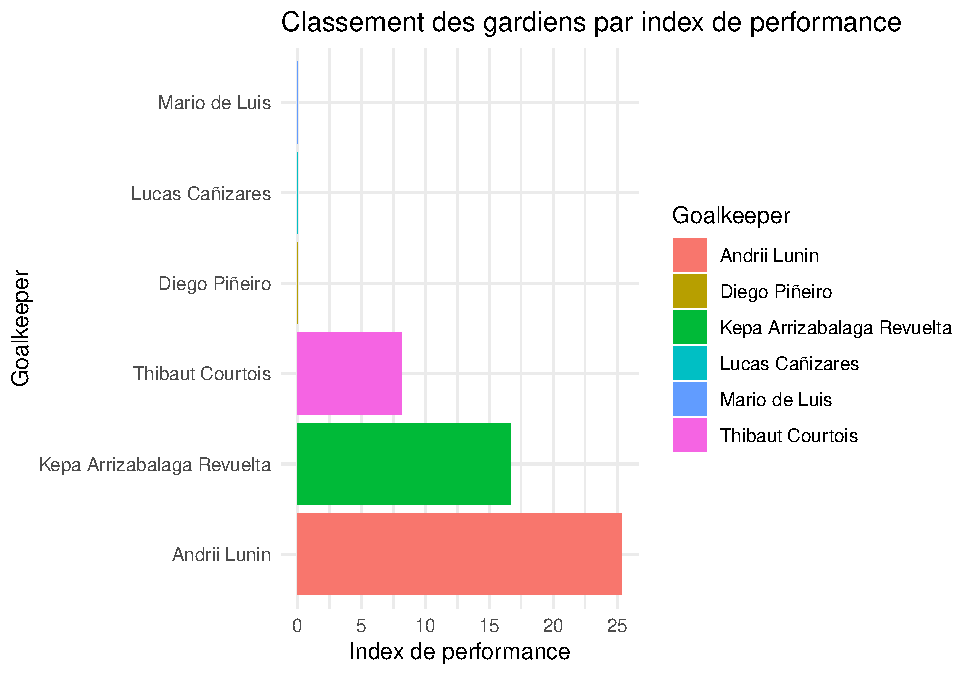
\includegraphics[width=0.8\linewidth]{Analyse_Impact_Performances_Joueurs_files/figure-latex/IndexPer - Gardiern-1}

\subsubsection{Index de Performance vs
Apparitions}\label{index-de-performance-vs-apparitions}

\begin{Shaded}
\begin{Highlighting}[]
\FunctionTok{library}\NormalTok{(ggplot2)             }\CommentTok{\# Load the package}

\FunctionTok{ggplot}\NormalTok{(GoalKeepers, }\FunctionTok{aes}\NormalTok{(}\AttributeTok{x =}\NormalTok{ appearances, }\AttributeTok{y =}\NormalTok{ performance\_index\_gk)) }\SpecialCharTok{+}
  \FunctionTok{geom\_line}\NormalTok{(}\AttributeTok{color =} \StringTok{"blue"}\NormalTok{, }\AttributeTok{group =} \DecValTok{1}\NormalTok{) }\SpecialCharTok{+}
  \FunctionTok{geom\_point}\NormalTok{(}\AttributeTok{size =} \DecValTok{3}\NormalTok{, }\FunctionTok{aes}\NormalTok{(}\AttributeTok{color =}\NormalTok{ name)) }\SpecialCharTok{+}  \CommentTok{\# Use colors for each goalkeeper}
  \FunctionTok{geom\_text}\NormalTok{(}\FunctionTok{aes}\NormalTok{(}\AttributeTok{label =}\NormalTok{ name), }\AttributeTok{vjust =} \SpecialCharTok{{-}}\DecValTok{1}\NormalTok{, }\AttributeTok{hjust =} \FloatTok{0.5}\NormalTok{, }\AttributeTok{size =} \DecValTok{3}\NormalTok{) }\SpecialCharTok{+}  \CommentTok{\# Add labels}
  \FunctionTok{labs}\NormalTok{(}
    \AttributeTok{title =} \StringTok{"Index de performance vs Apparitions"}\NormalTok{,}
    \AttributeTok{x =} \StringTok{"Nombre d\textquotesingle{}apparitions"}\NormalTok{,}
    \AttributeTok{y =} \StringTok{"Index de performance"}\NormalTok{,}
    \AttributeTok{color =} \StringTok{"Goalkeeper"}
\NormalTok{  ) }\SpecialCharTok{+}
  \FunctionTok{theme\_minimal}\NormalTok{()}
\end{Highlighting}
\end{Shaded}

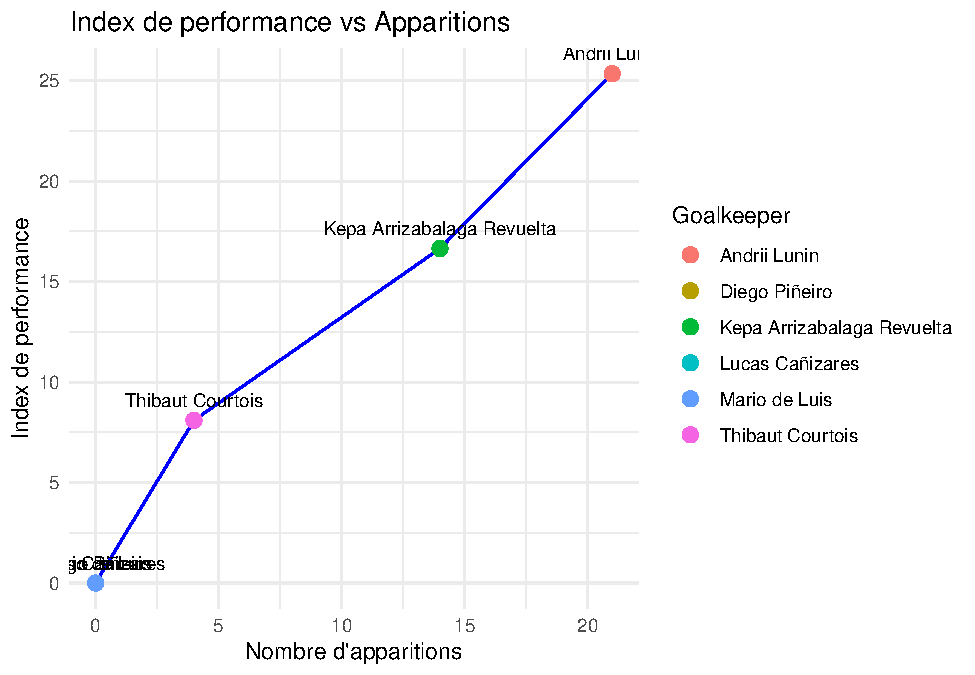
\includegraphics[width=0.8\linewidth]{Analyse_Impact_Performances_Joueurs_files/figure-latex/IndexPer vs Appar Gardiern-1}

\subsubsection{Distribution des Clean Sheets et Goals
Conceded}\label{distribution-des-clean-sheets-et-goals-conceded}

Ce bar plot compare les clean sheets et les buts concédés par chaque
gardien.

Les joueurs ayant un nombre élevé de clean sheets et un faible nombre de
buts concédés sont probablement les plus performants.

Si un joueur a peu d'apparitions mais un bon ratio de clean sheets, cela
pourrait indiquer une performance clé dans des matchs spécifiques, les
joueurs sans clean sheets et avec beaucoup de buts concédés peuvent
refléter une utilisation limitée ou des performances moins efficaces.

\begin{Shaded}
\begin{Highlighting}[]
\FunctionTok{library}\NormalTok{(tidyr)}
\FunctionTok{library}\NormalTok{(dplyr)}

\NormalTok{GoalKeepers\_long }\OtherTok{\textless{}{-}}\NormalTok{ GoalKeepers }\SpecialCharTok{\%\textgreater{}\%}
  \FunctionTok{mutate}\NormalTok{(}\AttributeTok{goals\_conceded =} \SpecialCharTok{{-}}\NormalTok{goals\_conceded) }\SpecialCharTok{\%\textgreater{}\%} 
  \FunctionTok{pivot\_longer}\NormalTok{(}\AttributeTok{cols =} \FunctionTok{c}\NormalTok{(clean\_sheets, goals\_conceded), }
               \AttributeTok{names\_to =} \StringTok{"metric"}\NormalTok{, }
               \AttributeTok{values\_to =} \StringTok{"value"}\NormalTok{)}

\CommentTok{\# Bar plot with goalkeeper names}
\FunctionTok{ggplot}\NormalTok{(GoalKeepers\_long, }\FunctionTok{aes}\NormalTok{(}\AttributeTok{x =}\NormalTok{ name, }\AttributeTok{y =}\NormalTok{ value, }\AttributeTok{fill =}\NormalTok{ metric)) }\SpecialCharTok{+}
  \FunctionTok{geom\_bar}\NormalTok{(}\AttributeTok{stat =} \StringTok{"identity"}\NormalTok{, }\AttributeTok{position =} \StringTok{"identity"}\NormalTok{, }\AttributeTok{alpha =} \FloatTok{0.7}\NormalTok{) }\SpecialCharTok{+}
  \FunctionTok{coord\_flip}\NormalTok{() }\SpecialCharTok{+}
  \FunctionTok{scale\_fill\_manual}\NormalTok{(}
    \AttributeTok{values =} \FunctionTok{c}\NormalTok{(}\StringTok{"clean\_sheets"} \OtherTok{=} \StringTok{"blue"}\NormalTok{, }\StringTok{"goals\_conceded"} \OtherTok{=} \StringTok{"red"}\NormalTok{),}
    \AttributeTok{labels =} \FunctionTok{c}\NormalTok{(}\StringTok{"Clean Sheets"}\NormalTok{, }\StringTok{"Goals Conceded"}\NormalTok{)}
\NormalTok{  ) }\SpecialCharTok{+}
  \FunctionTok{labs}\NormalTok{(}
    \AttributeTok{title =} \StringTok{"Comparaison des clean sheets et des buts concédés"}\NormalTok{,}
    \AttributeTok{x =} \StringTok{"Joueur"}\NormalTok{,}
    \AttributeTok{y =} \StringTok{"Nombre"}\NormalTok{,}
    \AttributeTok{fill =} \StringTok{"Légende"}
\NormalTok{  ) }\SpecialCharTok{+}
  \FunctionTok{geom\_text}\NormalTok{(}\FunctionTok{aes}\NormalTok{(}\AttributeTok{label =} \FunctionTok{ifelse}\NormalTok{(value }\SpecialCharTok{!=} \DecValTok{0}\NormalTok{, }\FunctionTok{paste0}\NormalTok{(value), }\StringTok{""}\NormalTok{)), }
            \AttributeTok{position =} \FunctionTok{position\_stack}\NormalTok{(}\AttributeTok{vjust =} \FloatTok{0.5}\NormalTok{), }\AttributeTok{size =} \DecValTok{3}\NormalTok{) }\SpecialCharTok{+}
  \FunctionTok{theme\_minimal}\NormalTok{()}
\end{Highlighting}
\end{Shaded}

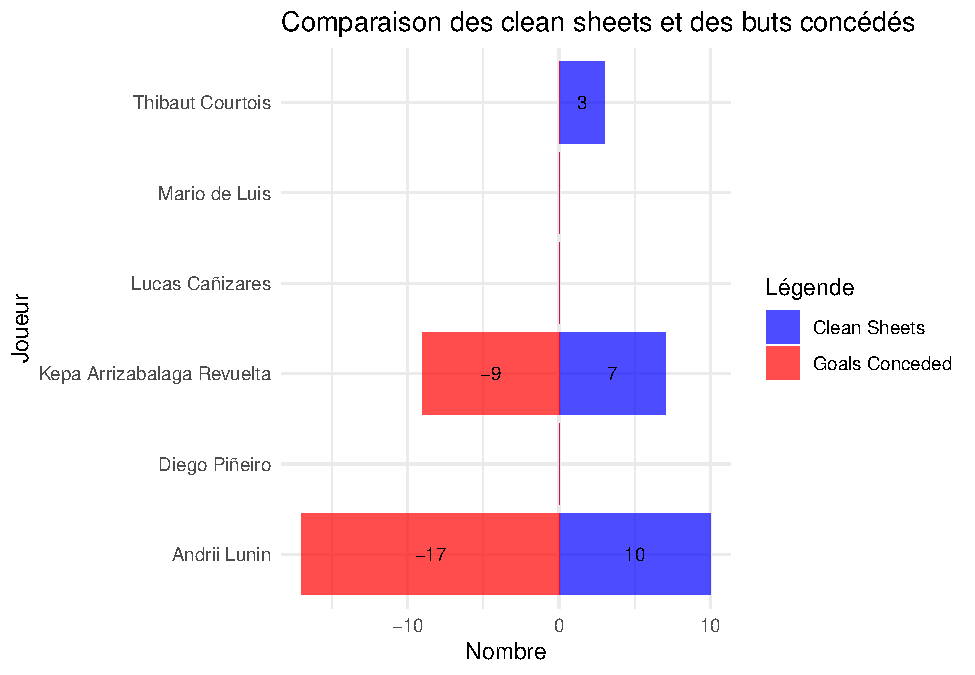
\includegraphics[width=0.8\linewidth]{Analyse_Impact_Performances_Joueurs_files/figure-latex/DistributionGardiern-1}

\subsubsection{Taux de Réussite des
Distributions}\label{taux-de-ruxe9ussite-des-distributions}

Ce nuage de points analyse la relation entre les distributions réussies
et échouées des gardiens.

Le taux de réussite montre l'efficacité de chaque joueur dans la
distribution du ballon.

Les gardiens avec des taux élevés, visibles dans les tons verts,
démontrent une grande précision, essentielle pour maintenir le contrôle
du jeu.

\includegraphics[width=0.8\linewidth]{Analyse_Impact_Performances_Joueurs_files/figure-latex/Taux de RéussiteGardiern-1}

\subsubsection{Saves Made vs Goals
Conceded}\label{saves-made-vs-goals-conceded}

Ce graphique illustre la corrélation entre les arrêts réalisés (saves
made) et les buts encaissés (goals conceded) par les gardiens.

Il est clair dans l'ensemble que les gardiens qui réalisent plus
d'arrêts ont tendance à encaisser plus de buts, comme le montre la ligne
de régression.

\begin{verbatim}
## `geom_smooth()` using formula = 'y ~ x'
\end{verbatim}

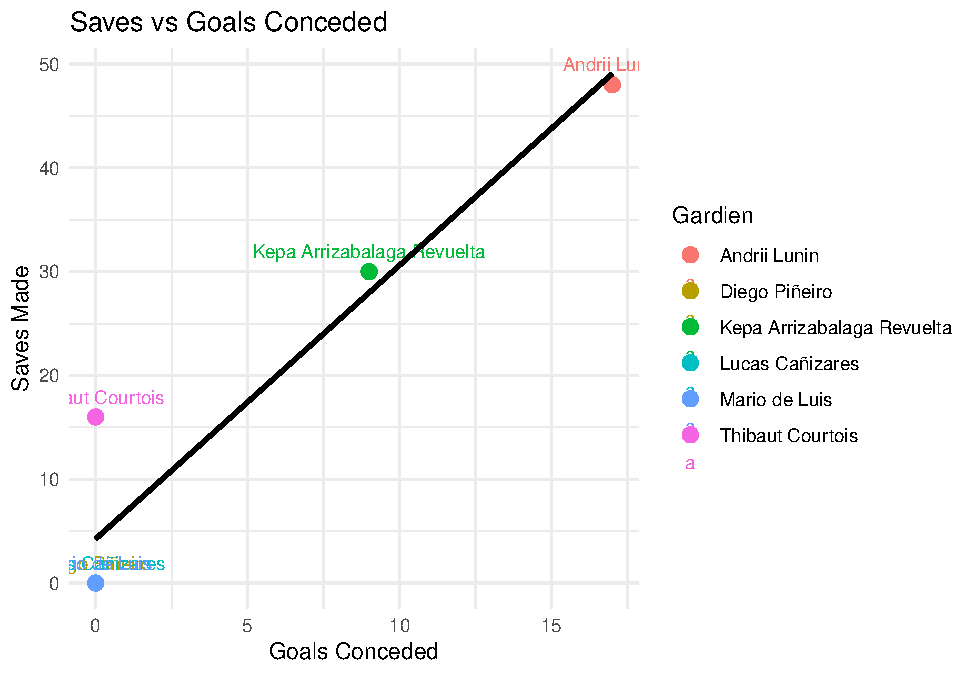
\includegraphics[width=0.8\linewidth]{Analyse_Impact_Performances_Joueurs_files/figure-latex/SavesVsBEGardiern-1}

\subsubsection{Clustering Goalkeepers Based on Performance
Metrics}\label{clustering-goalkeepers-based-on-performance-metrics}

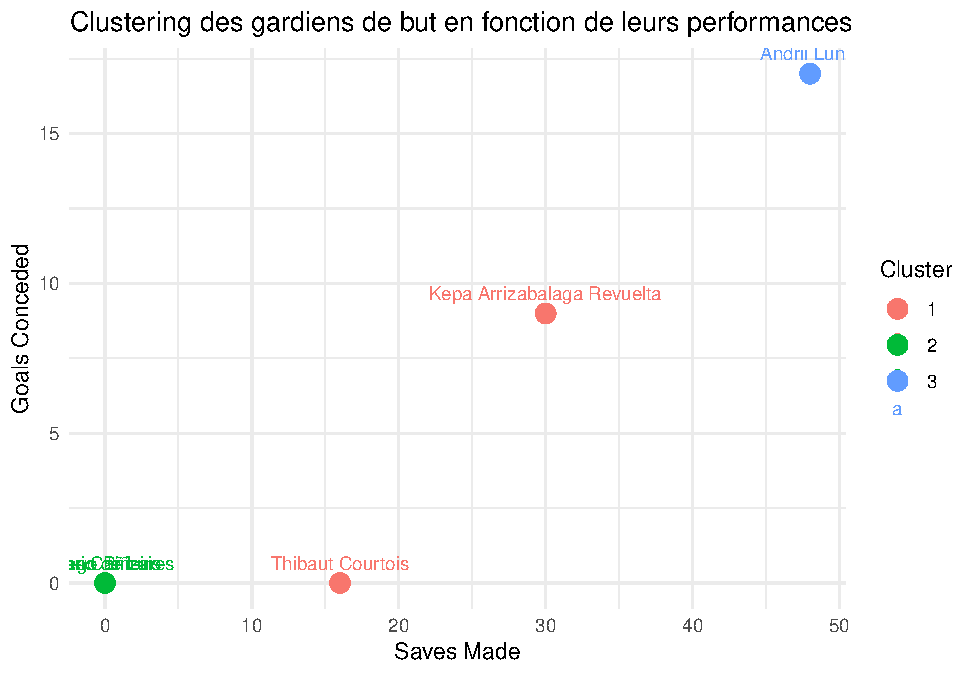
\includegraphics[width=0.8\linewidth]{Analyse_Impact_Performances_Joueurs_files/figure-latex/clustering-1}

\subsection{Defenders performance
index}\label{defenders-performance-index}

Le classement des défenseurs selon leur index de performance met en
avant José Ignacio Fernández Iglesias comme le joueur ayant obtenu le
score le plus élevé, suivi par Dani Carvajal et Antonio Rüdiger.

Ces résultats suggèrent que ces joueurs ont excellé dans plusieurs
catégories clés, telles que les interventions défensives (interceptions,
blocs) et leur contribution aux clean sheets.

À l'opposé, des joueurs comme Vinícius Augusto Tobias da Silva et Jacobo
Ramón affichent des scores relativement faibles, ce qui pourrait
refléter un manque d'implication ou une participation limitée dans les
matchs joués.

Les paramètres ayant un impact négatif important, tels que les buts
encaissés et les buts contre leur camp (own goals), semblent avoir
significativement diminué les performances de certains défenseurs.
Cependant, les actions décisives, telles que les dégagements sur la
ligne et les buts marqués, ont un effet très bénéfique sur l'index

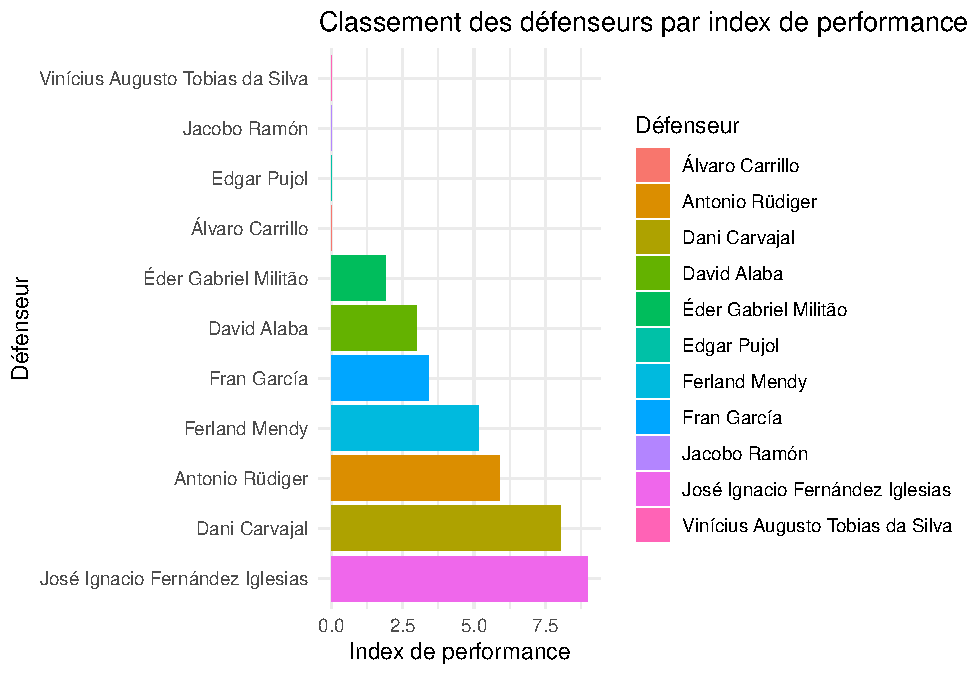
\includegraphics[width=0.8\linewidth]{Analyse_Impact_Performances_Joueurs_files/figure-latex/Defenders performance index-1}

\subsubsection{Clean sheat ratio}\label{clean-sheat-ratio}

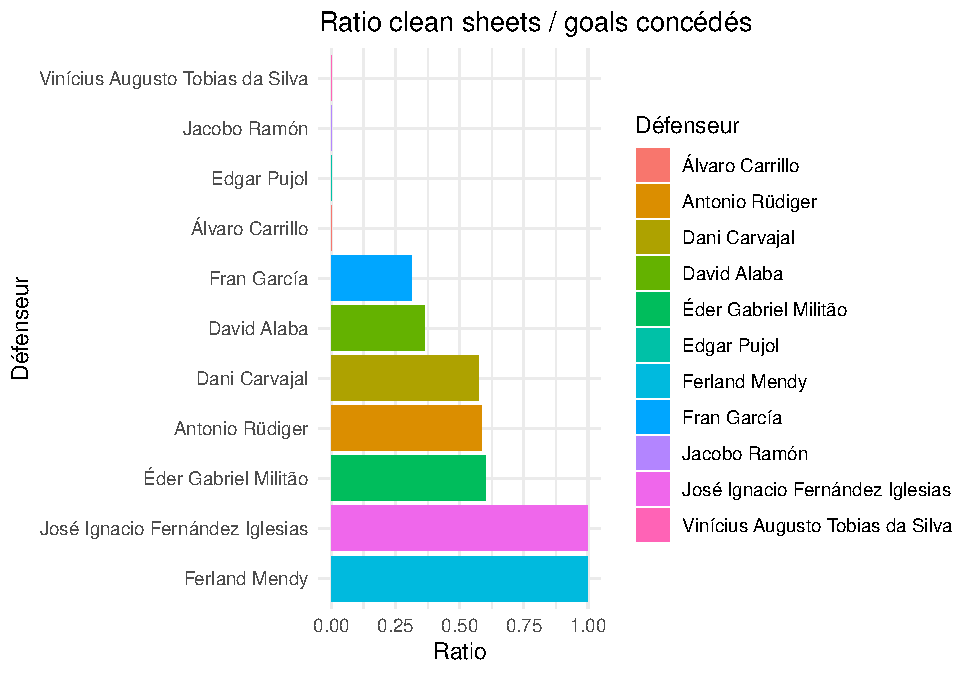
\includegraphics[width=0.8\linewidth]{Analyse_Impact_Performances_Joueurs_files/figure-latex/Clean sheat ratio-def-1}

\subsubsection{Correlation entre Clean Sheets et Goals
Conceded}\label{correlation-entre-clean-sheets-et-goals-conceded}

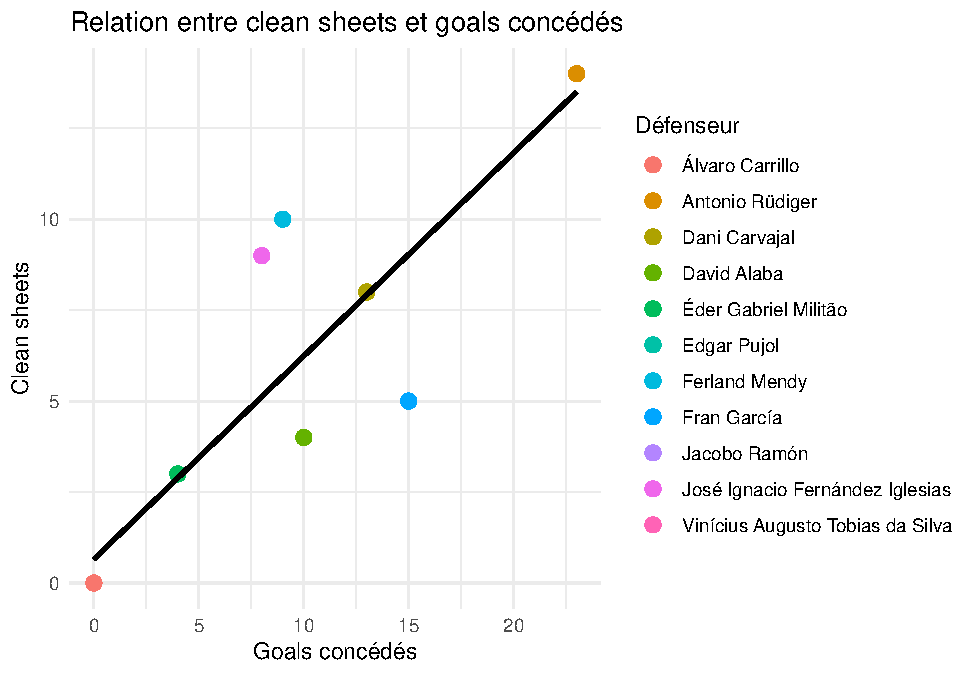
\includegraphics[width=0.8\linewidth]{Analyse_Impact_Performances_Joueurs_files/figure-latex/CorrelationCleansheets et goalsconceded-def-1}

\subsubsection{Corrélation entre l'index de performance et les
différentes
statistiques}\label{corruxe9lation-entre-lindex-de-performance-et-les-diffuxe9rentes-statistiques}

La matrice de corrélation montre les relations entre l'index de
performance des défenseurs et plusieurs métriques clés. On observe une
forte corrélation positive entre l'index de performance et les variables
suivantes :

\begin{itemize}
\tightlist
\item
  Appearances (appearances) : r = 0.92
\end{itemize}

ce qui indique que les joueurs qui participent à plus de matchs ont
tendance à avoir un index de performance plus élevé.

\begin{itemize}
\tightlist
\item
  Clean sheets : r = 0.86
\end{itemize}

suggérant que les performances défensives solides (sans buts encaissés)
contribuent grandement à un bon score.

\begin{itemize}
\tightlist
\item
  Clearances off the line (dégagements sur la ligne) : = 0.87
\end{itemize}

ce qui reflète l'importance des actions défensives décisives.

\begin{itemize}
\tightlist
\item
  Blocs : r = 0.76
\end{itemize}

confirmant leur rôle essentiel dans la réduction des opportunités
adverses.

Par contre, on constate une corrélation négative pour :

\begin{itemize}
\tightlist
\item
  Goals conceded (buts encaissés) : r = −0.86
\end{itemize}

indiquant que les buts encaissés diminuent fortement l'index de
performance.

\begin{itemize}
\tightlist
\item
  Own goals scored (buts contre son camp) : r = −0.03
\end{itemize}

montrant un effet légèrement négatif mais moins significatif.

\begin{Shaded}
\begin{Highlighting}[]
\NormalTok{cor\_matrix }\OtherTok{\textless{}{-}} \FunctionTok{cor}\NormalTok{(Defenders[, }\FunctionTok{c}\NormalTok{(}\StringTok{"appearances"}\NormalTok{, }\StringTok{"blocks"}\NormalTok{, }\StringTok{"clean\_sheets"}\NormalTok{, }\StringTok{"clearances\_off\_the\_line"}\NormalTok{, }\StringTok{"goals"}\NormalTok{, }
                                \StringTok{"goals\_conceded"}\NormalTok{, }\StringTok{"interceptions"}\NormalTok{, }\StringTok{"own\_goal\_scored"}\NormalTok{, }\StringTok{"performance\_index\_def"}\NormalTok{)], }
                  \AttributeTok{use =} \StringTok{"complete.obs"}\NormalTok{)}

\FunctionTok{library}\NormalTok{(ggcorrplot)}
\FunctionTok{ggcorrplot}\NormalTok{(cor\_matrix, }\AttributeTok{method =} \StringTok{"circle"}\NormalTok{, }\AttributeTok{type =} \StringTok{"lower"}\NormalTok{, }\AttributeTok{lab =} \ConstantTok{TRUE}\NormalTok{, }\AttributeTok{lab\_size =} \DecValTok{3}\NormalTok{, }\AttributeTok{colors =} \FunctionTok{c}\NormalTok{(}\StringTok{"red"}\NormalTok{, }\StringTok{"white"}\NormalTok{, }\StringTok{"blue"}\NormalTok{))}
\end{Highlighting}
\end{Shaded}

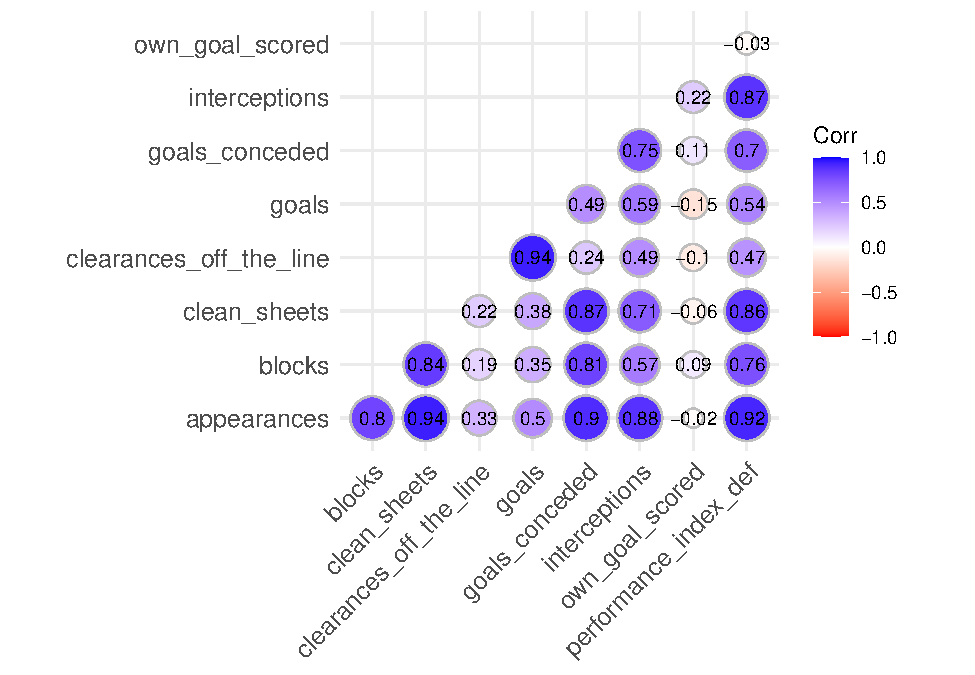
\includegraphics[width=0.8\linewidth]{Analyse_Impact_Performances_Joueurs_files/figure-latex/Correlation indexPerformance et diff stat-def-1}

\subsubsection{Clustering des défenseurs en fonction de l'index de
performance et d'autres
métriques}\label{clustering-des-duxe9fenseurs-en-fonction-de-lindex-de-performance-et-dautres-muxe9triques}

\begin{Shaded}
\begin{Highlighting}[]
\NormalTok{clustering\_data }\OtherTok{\textless{}{-}}\NormalTok{ Defenders }\SpecialCharTok{\%\textgreater{}\%}
  \FunctionTok{select}\NormalTok{(performance\_index\_def, interceptions, blocks) }\SpecialCharTok{\%\textgreater{}\%}
  \FunctionTok{scale}\NormalTok{()}

\CommentTok{\# Clustering K{-}means}
\FunctionTok{set.seed}\NormalTok{(}\DecValTok{123}\NormalTok{)}
\NormalTok{kmeans\_result }\OtherTok{\textless{}{-}} \FunctionTok{kmeans}\NormalTok{(clustering\_data, }\AttributeTok{centers =} \DecValTok{3}\NormalTok{, }\AttributeTok{nstart =} \DecValTok{20}\NormalTok{)}
\NormalTok{Defenders}\SpecialCharTok{$}\NormalTok{cluster }\OtherTok{\textless{}{-}} \FunctionTok{as.factor}\NormalTok{(kmeans\_result}\SpecialCharTok{$}\NormalTok{cluster)}

\CommentTok{\# Visualisation des clusters}
\FunctionTok{ggplot}\NormalTok{(Defenders, }\FunctionTok{aes}\NormalTok{(}\AttributeTok{x =}\NormalTok{ interceptions, }\AttributeTok{y =}\NormalTok{ blocks, }\AttributeTok{color =}\NormalTok{ cluster)) }\SpecialCharTok{+}
  \FunctionTok{geom\_point}\NormalTok{(}\AttributeTok{size =} \DecValTok{4}\NormalTok{) }\SpecialCharTok{+}
  \FunctionTok{geom\_text}\NormalTok{(}\FunctionTok{aes}\NormalTok{(}\AttributeTok{label =}\NormalTok{ name), }\AttributeTok{vjust =} \SpecialCharTok{{-}}\DecValTok{1}\NormalTok{, }\AttributeTok{size =} \DecValTok{3}\NormalTok{) }\SpecialCharTok{+}
  \FunctionTok{labs}\NormalTok{(}
    \AttributeTok{title =} \StringTok{"Clustering des défenseurs en fonction des performances"}\NormalTok{,}
    \AttributeTok{x =} \StringTok{"Interceptions"}\NormalTok{,}
    \AttributeTok{y =} \StringTok{"Blocks"}\NormalTok{,}
    \AttributeTok{color =} \StringTok{"Cluster"}
\NormalTok{  ) }\SpecialCharTok{+}
  \FunctionTok{theme\_minimal}\NormalTok{()}
\end{Highlighting}
\end{Shaded}

\includegraphics[width=0.8\linewidth]{Analyse_Impact_Performances_Joueurs_files/figure-latex/Comparaison des passes réussies-def-1}

\subsubsection{Top 5 défenseurs par index de
performance}\label{top-5-duxe9fenseurs-par-index-de-performance}

\begin{Shaded}
\begin{Highlighting}[]
\NormalTok{top\_5\_defenders }\OtherTok{\textless{}{-}}\NormalTok{ Defenders }\SpecialCharTok{\%\textgreater{}\%}
  \FunctionTok{arrange}\NormalTok{(}\FunctionTok{desc}\NormalTok{(performance\_index\_def)) }\SpecialCharTok{\%\textgreater{}\%}
  \FunctionTok{head}\NormalTok{(}\DecValTok{5}\NormalTok{)}

\CommentTok{\# Visualisation des 5 meilleurs défenseurs}
\FunctionTok{ggplot}\NormalTok{(top\_5\_defenders, }\FunctionTok{aes}\NormalTok{(}\AttributeTok{x =} \FunctionTok{reorder}\NormalTok{(name, }\SpecialCharTok{{-}}\NormalTok{performance\_index\_def), }\AttributeTok{y =}\NormalTok{ performance\_index\_def, }\AttributeTok{fill =}\NormalTok{ name)) }\SpecialCharTok{+}
  \FunctionTok{geom\_bar}\NormalTok{(}\AttributeTok{stat =} \StringTok{"identity"}\NormalTok{) }\SpecialCharTok{+}
  \FunctionTok{coord\_flip}\NormalTok{() }\SpecialCharTok{+}
  \FunctionTok{labs}\NormalTok{(}
    \AttributeTok{title =} \StringTok{"Top 5 défenseurs par index de performance"}\NormalTok{,}
    \AttributeTok{x =} \StringTok{"Défenseur"}\NormalTok{,}
    \AttributeTok{y =} \StringTok{"Index de performance"}\NormalTok{,}
    \AttributeTok{fill =} \StringTok{"Défenseur"}
\NormalTok{  ) }\SpecialCharTok{+}
  \FunctionTok{theme\_minimal}\NormalTok{()}
\end{Highlighting}
\end{Shaded}

\begin{center}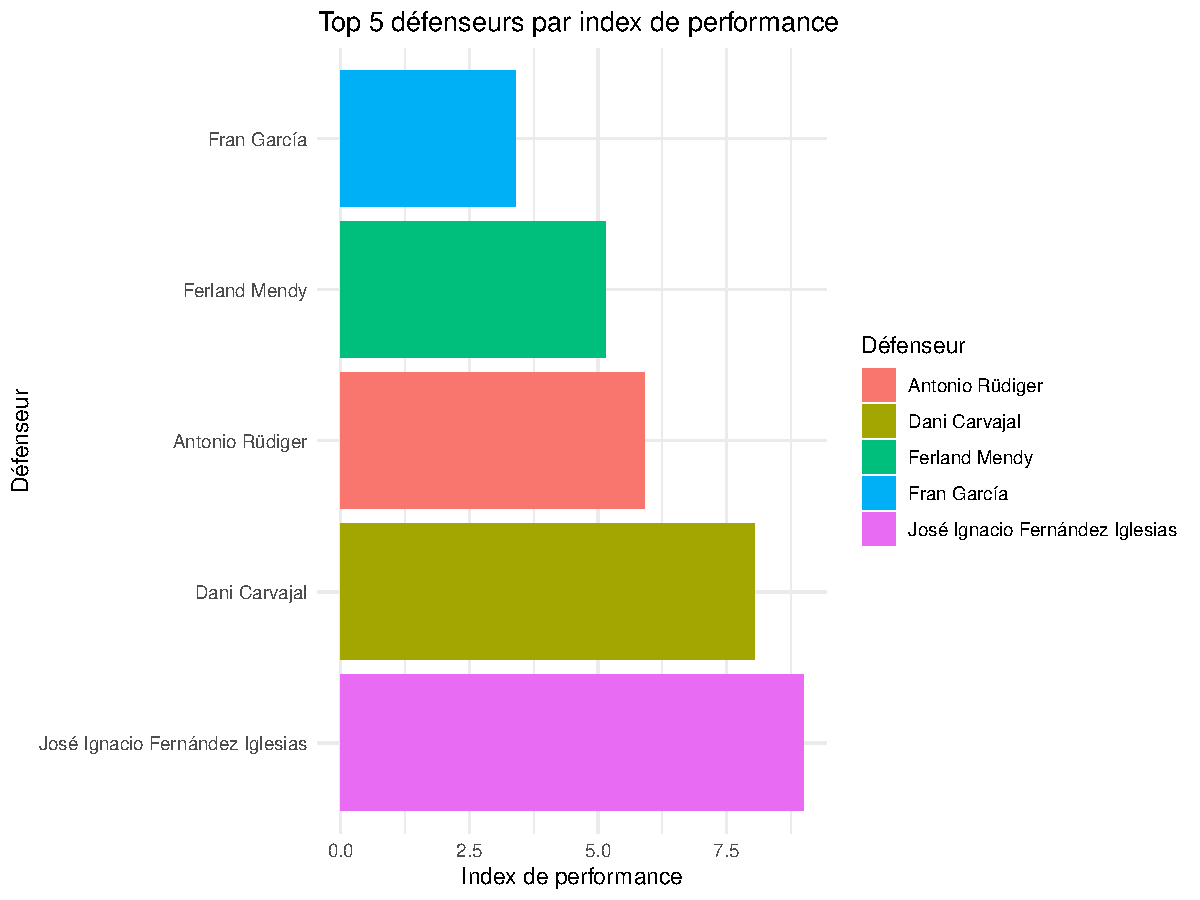
\includegraphics[width=0.8\linewidth]{Analyse_Impact_Performances_Joueurs_files/figure-latex/Top5-def-1} \end{center}

\subsubsection{Contribution des Clean Sheets par
Défenseur}\label{contribution-des-clean-sheets-par-duxe9fenseur}

\begin{center}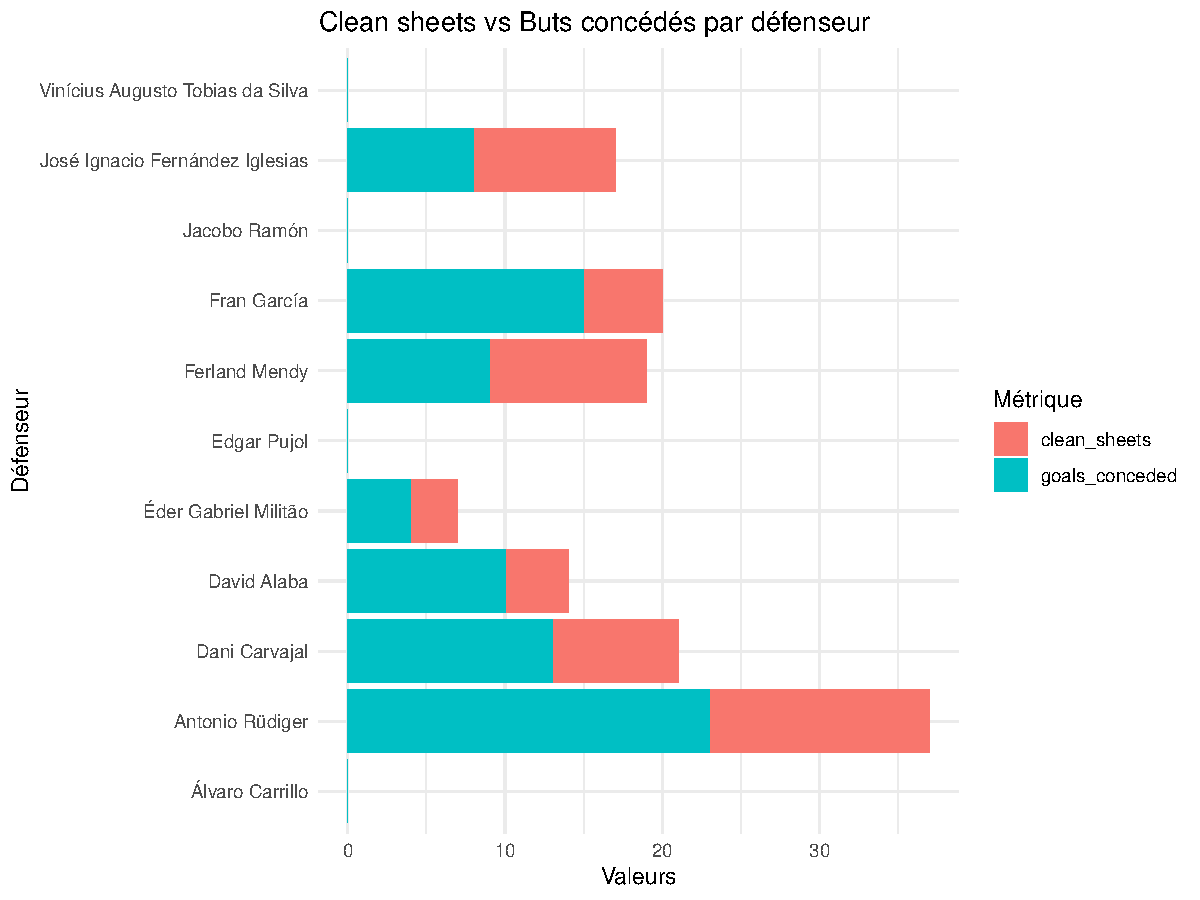
\includegraphics[width=0.8\linewidth]{Analyse_Impact_Performances_Joueurs_files/figure-latex/Contribution-def-1} \end{center}

\subsection{Midfielders performance
index}\label{midfielders-performance-index}

Le classement des milieux de terrain en fonction de leur index de
performance montre clairement que Toni Kroos occupe la première place,
suivi de Federico Valverde et Luka Modric.

Ces résultats reflètent leur forte contribution dans les domaines clés
tels que les passes décisives (goal assists), les passes clés (key
passes), et les buts marqués.

Ces métriques ayant des pondérations élevées dans la formule, elles
jouent un rôle déterminant dans leurs scores élevés

\begin{center}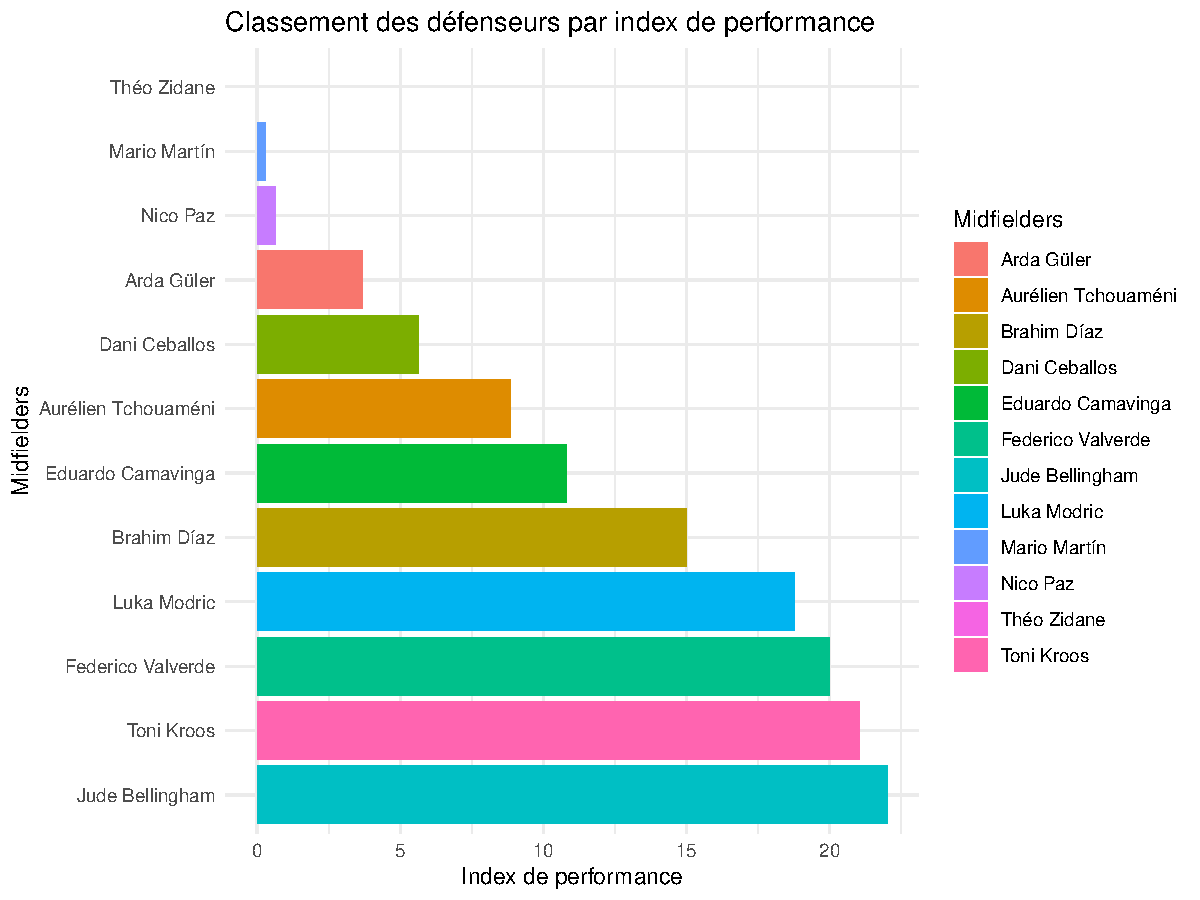
\includegraphics[width=0.8\linewidth]{Analyse_Impact_Performances_Joueurs_files/figure-latex/performance index-mid-1} \end{center}

\begin{verbatim}
##  [1] -1.85 -3.50 -8.85 -2.40 -6.90 -4.95 -9.50 -4.75 -0.10 -0.25  0.00 -3.35
##  [1]  -2.1  -9.2  -8.2  -3.9  -9.0 -14.3 -14.3 -11.3  -0.3  -0.5   0.0  -8.8
\end{verbatim}

\subsubsection{Contribution aux Buts (Goals +
Assists)}\label{contribution-aux-buts-goals-assists}

\begin{center}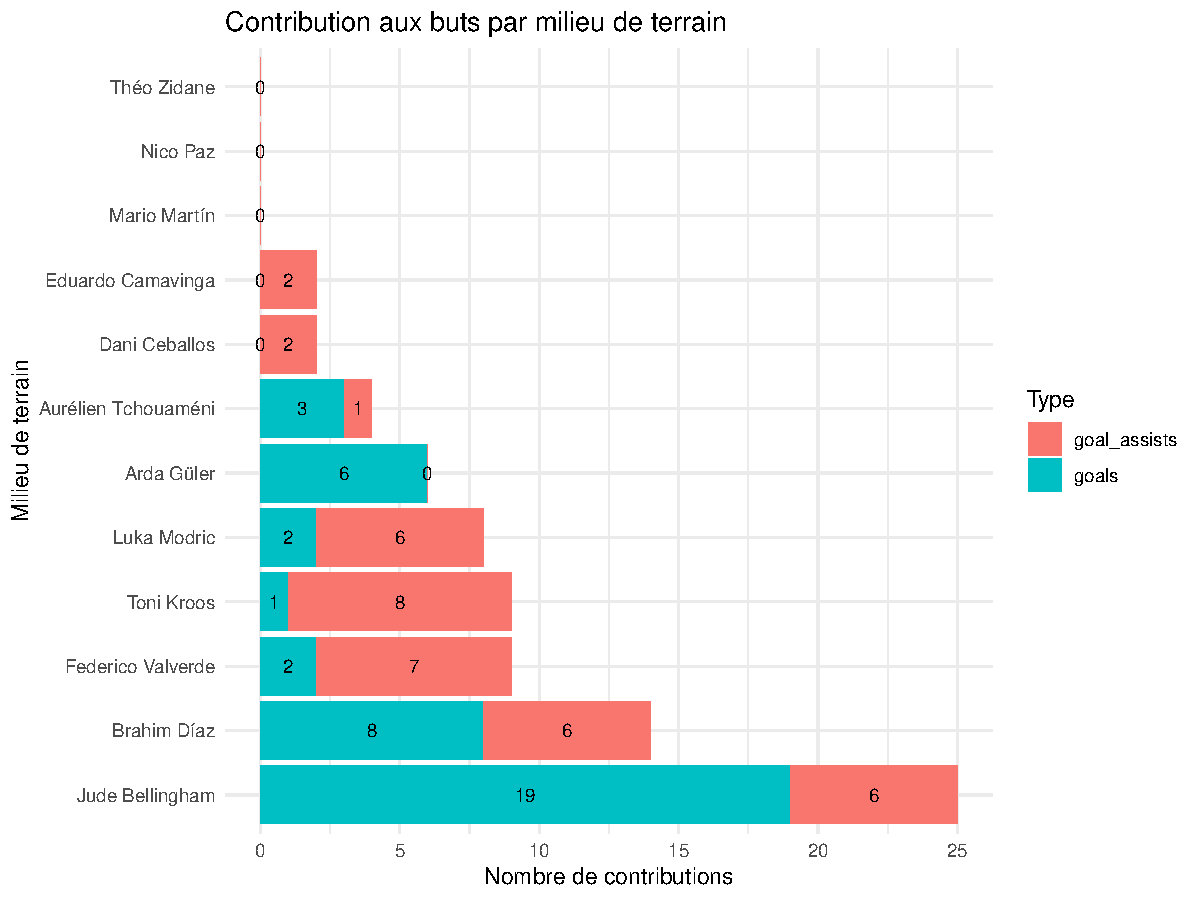
\includegraphics[width=0.8\linewidth]{Analyse_Impact_Performances_Joueurs_files/figure-latex/Contribution buts et assits-mid-1} \end{center}

\subsubsection{Correlation entre les
Metriques}\label{correlation-entre-les-metriques}

\begin{Shaded}
\begin{Highlighting}[]
\NormalTok{cor\_matrix }\OtherTok{\textless{}{-}} \FunctionTok{cor}\NormalTok{(Midfielders[, }\FunctionTok{c}\NormalTok{(}\StringTok{"appearances"}\NormalTok{, }\StringTok{"assists\_intentional"}\NormalTok{, }\StringTok{"goal\_assists"}\NormalTok{, }\StringTok{"goals"}\NormalTok{, }
                                  \StringTok{"key\_passes\_attempt\_assists"}\NormalTok{, }\StringTok{"performance\_index\_mid"}\NormalTok{)])}


\FunctionTok{library}\NormalTok{(ggcorrplot)}
\FunctionTok{ggcorrplot}\NormalTok{(cor\_matrix, }\AttributeTok{method =} \StringTok{"circle"}\NormalTok{, }\AttributeTok{type =} \StringTok{"lower"}\NormalTok{, }\AttributeTok{lab =} \ConstantTok{TRUE}\NormalTok{, }\AttributeTok{lab\_size =} \DecValTok{3}\NormalTok{, }
           \AttributeTok{colors =} \FunctionTok{c}\NormalTok{(}\StringTok{"red"}\NormalTok{, }\StringTok{"white"}\NormalTok{, }\StringTok{"blue"}\NormalTok{)) }\SpecialCharTok{+}
  \FunctionTok{labs}\NormalTok{(}\AttributeTok{title =} \StringTok{"Corrélations entre les métriques des milieux"}\NormalTok{)}
\end{Highlighting}
\end{Shaded}

\begin{center}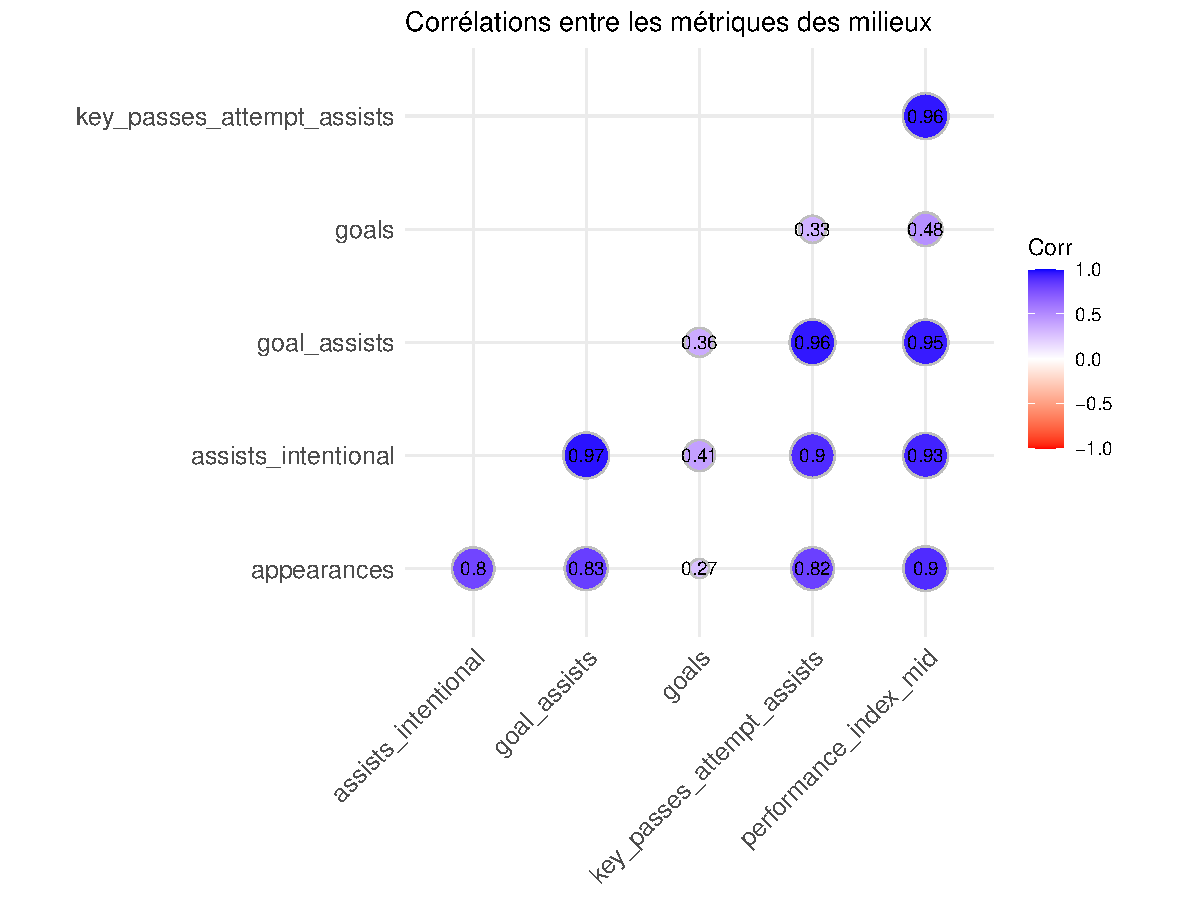
\includegraphics[width=0.8\linewidth]{Analyse_Impact_Performances_Joueurs_files/figure-latex/Correlations-mid-1} \end{center}

\subsubsection{Joueurs les plus
constants}\label{joueurs-les-plus-constants}

Le graphique compare les performances individuelles des milieux de
terrain en se basant sur trois métriques normalisées : les passes
décisives (goal assists), les buts marqués (goals), et les passes clés
tentées (key passes attempt assists).

\begin{itemize}
\item
  Jude Bellingham, bien qu'il occupe une position de milieu de terrain,
  se distingue par ses performances constantes et exceptionnelles, tant
  en termes de buts marqués que de passes décisives. Cette polyvalence
  offensive le place parmi les joueurs les plus influents, démontrant sa
  capacité à contribuer de manière significative à l'attaque tout en
  assurant son rôle au milieu du terrain.
\item
  Toni Kroos et Luka Modric se démarquent comme les joueurs les plus
  constants sur l'ensemble des métriques, atteignant des valeurs élevées
  dans presque toutes les catégories.
\item
  Federico Valverde présente une performance solide, notamment dans les
  buts marqués et les passes clés, mais légèrement inférieure en passes
  décisives.
\end{itemize}

À l'inverse, des joueurs comme Théo Zidane, Mario Martín, et Nico Paz
affichent des valeurs normalisées faibles, ce qui pourrait refléter une
contribution limitée ou faible implications dans les matchs.

Une diversité de styles de jeu est observable : certains joueurs comme
Arda Güler se concentrent davantage sur des aspects spécifiques, tandis
que d'autres, comme Eduardo Camavinga, ont des performances plus
équilibrées.

\begin{itemize}
\tightlist
\item
  Ce graphique met en évidence les différences de contributions entre
  les milieux de terrain. Les joueurs expérimentés comme Kroos et Modric
  dominent grâce à leur régularité et leur influence dans plusieurs
  domaines du jeu, tandis que les jeunes joueurs ou ceux moins impliqués
  présentent des performances plus spécialisées ou limitées. Cette
  visualisation peut être utilisée pour identifier les points forts
  spécifiques de chaque joueur et optimiser leur rôle sur le terrain.
\end{itemize}

\begin{Shaded}
\begin{Highlighting}[]
\NormalTok{Midfielders\_norm }\OtherTok{\textless{}{-}}\NormalTok{ Midfielders }\SpecialCharTok{\%\textgreater{}\%}
  \FunctionTok{mutate}\NormalTok{(}\FunctionTok{across}\NormalTok{(}\FunctionTok{c}\NormalTok{(goals, goal\_assists, key\_passes\_attempt\_assists), }\SpecialCharTok{\textasciitilde{}}\NormalTok{ . }\SpecialCharTok{/} \FunctionTok{max}\NormalTok{(.), }\AttributeTok{.names =} \StringTok{"norm\_\{.col\}"}\NormalTok{))}

\CommentTok{\# Boxplot pour les métriques normalisées}
\NormalTok{Midfielders\_long }\OtherTok{\textless{}{-}}\NormalTok{ Midfielders\_norm }\SpecialCharTok{\%\textgreater{}\%}
  \FunctionTok{pivot\_longer}\NormalTok{(}\AttributeTok{cols =} \FunctionTok{starts\_with}\NormalTok{(}\StringTok{"norm"}\NormalTok{), }\AttributeTok{names\_to =} \StringTok{"metric"}\NormalTok{, }\AttributeTok{values\_to =} \StringTok{"value"}\NormalTok{)}

\CommentTok{\# Calculer un score total normalisé}

\CommentTok{\# Diagramme en barres pour les scores totaux}
\FunctionTok{ggplot}\NormalTok{(Midfielders\_long, }\FunctionTok{aes}\NormalTok{(}\AttributeTok{x =}\NormalTok{ metric, }\AttributeTok{y =}\NormalTok{ value, }\AttributeTok{color =}\NormalTok{ name, }\AttributeTok{group =}\NormalTok{ name)) }\SpecialCharTok{+}
  \FunctionTok{geom\_line}\NormalTok{() }\SpecialCharTok{+}
  \FunctionTok{geom\_point}\NormalTok{(}\AttributeTok{size =} \DecValTok{3}\NormalTok{) }\SpecialCharTok{+}
  \FunctionTok{labs}\NormalTok{(}
    \AttributeTok{title =} \StringTok{"Comparaison des performances individuelles"}\NormalTok{,}
    \AttributeTok{x =} \StringTok{"Métrique"}\NormalTok{,}
    \AttributeTok{y =} \StringTok{"Valeur normalisée"}\NormalTok{,}
    \AttributeTok{color =} \StringTok{"Milieu"}
\NormalTok{  ) }\SpecialCharTok{+}
  \FunctionTok{theme\_minimal}\NormalTok{()}
\end{Highlighting}
\end{Shaded}

\begin{center}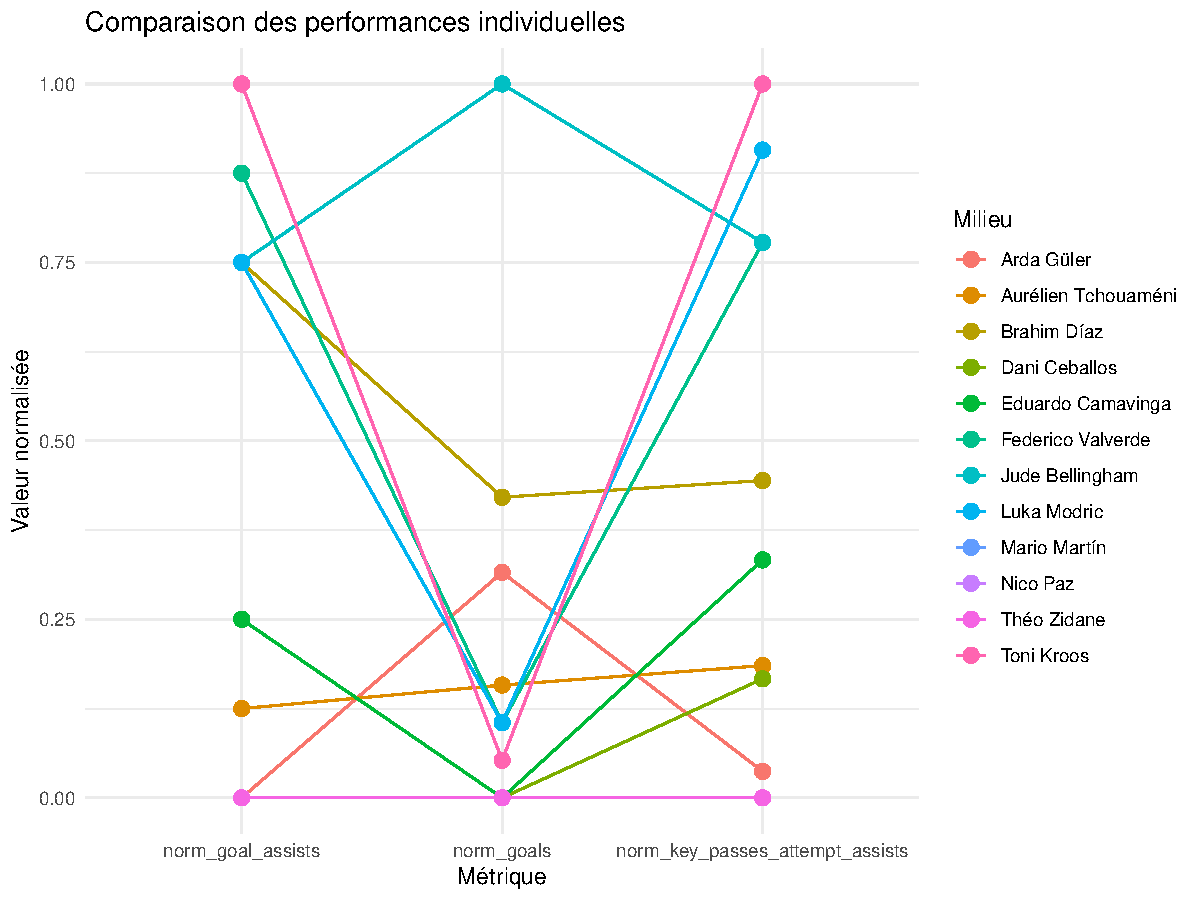
\includegraphics[width=0.8\linewidth]{Analyse_Impact_Performances_Joueurs_files/figure-latex/constans-mid-1} \end{center}

\subsubsection{Clustering par
performance}\label{clustering-par-performance}

\begin{Shaded}
\begin{Highlighting}[]
\NormalTok{clustering\_data }\OtherTok{\textless{}{-}}\NormalTok{ Midfielders }\SpecialCharTok{\%\textgreater{}\%}
  \FunctionTok{select}\NormalTok{(goals, goal\_assists, key\_passes\_attempt\_assists, performance\_index\_mid) }\SpecialCharTok{\%\textgreater{}\%}
  \FunctionTok{scale}\NormalTok{()}

\CommentTok{\# K{-}means clustering}
\FunctionTok{set.seed}\NormalTok{(}\DecValTok{123}\NormalTok{)}
\NormalTok{kmeans\_result }\OtherTok{\textless{}{-}} \FunctionTok{kmeans}\NormalTok{(clustering\_data, }\AttributeTok{centers =} \DecValTok{3}\NormalTok{, }\AttributeTok{nstart =} \DecValTok{20}\NormalTok{)}
\NormalTok{Midfielders}\SpecialCharTok{$}\NormalTok{cluster }\OtherTok{\textless{}{-}} \FunctionTok{as.factor}\NormalTok{(kmeans\_result}\SpecialCharTok{$}\NormalTok{cluster)}

\CommentTok{\# Visualiser les clusters}
\FunctionTok{ggplot}\NormalTok{(Midfielders, }\FunctionTok{aes}\NormalTok{(}\AttributeTok{x =}\NormalTok{ goals, }\AttributeTok{y =}\NormalTok{ performance\_index\_mid, }\AttributeTok{color =}\NormalTok{ cluster)) }\SpecialCharTok{+}
  \FunctionTok{geom\_point}\NormalTok{(}\AttributeTok{size =} \DecValTok{4}\NormalTok{) }\SpecialCharTok{+}
  \FunctionTok{geom\_text}\NormalTok{(}\FunctionTok{aes}\NormalTok{(}\AttributeTok{label =}\NormalTok{ name), }\AttributeTok{vjust =} \SpecialCharTok{{-}}\DecValTok{1}\NormalTok{, }\AttributeTok{size =} \DecValTok{3}\NormalTok{) }\SpecialCharTok{+}
  \FunctionTok{labs}\NormalTok{(}
    \AttributeTok{title =} \StringTok{"Clustering des milieux en fonction des performances"}\NormalTok{,}
    \AttributeTok{x =} \StringTok{"Buts"}\NormalTok{,}
    \AttributeTok{y =} \StringTok{"Index de performance"}\NormalTok{,}
    \AttributeTok{color =} \StringTok{"Cluster"}
\NormalTok{  ) }\SpecialCharTok{+}
  \FunctionTok{theme\_minimal}\NormalTok{()}
\end{Highlighting}
\end{Shaded}

\begin{center}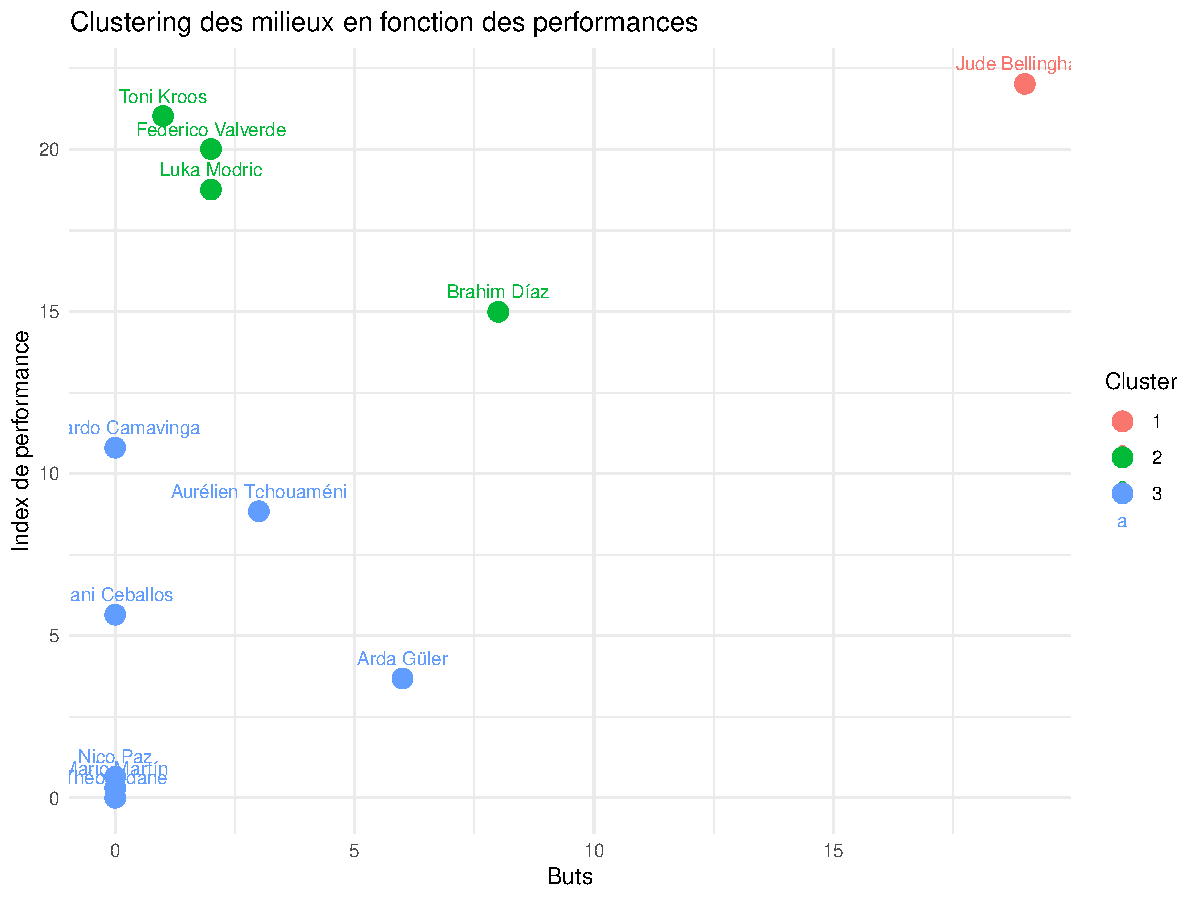
\includegraphics[width=0.8\linewidth]{Analyse_Impact_Performances_Joueurs_files/figure-latex/Clustering-mid-1} \end{center}

\subsection{Forwards performance
index}\label{forwards-performance-index}

\begin{Shaded}
\begin{Highlighting}[]
\NormalTok{Forwards}\SpecialCharTok{$}\NormalTok{shots\_off\_targets }\OtherTok{\textless{}{-}}\NormalTok{ Forwards}\SpecialCharTok{$}\NormalTok{total\_shots }\SpecialCharTok{{-}}\NormalTok{ (  Forwards}\SpecialCharTok{$}\NormalTok{shots\_on\_target\_inc\_goals)}
\NormalTok{Forwards}\SpecialCharTok{$}\NormalTok{penalties\_missed }\OtherTok{\textless{}{-}}\NormalTok{ Forwards}\SpecialCharTok{$}\NormalTok{penalties\_taken }\SpecialCharTok{{-}}\NormalTok{ Forwards}\SpecialCharTok{$}\NormalTok{penalty\_goals}


\NormalTok{Forwards}\SpecialCharTok{$}\NormalTok{performance\_index\_fw }\OtherTok{\textless{}{-}} 
\NormalTok{  Forwards}\SpecialCharTok{$}\NormalTok{appearances }\SpecialCharTok{*} \FloatTok{0.1} \SpecialCharTok{+} 
\NormalTok{  Forwards}\SpecialCharTok{$}\NormalTok{goal\_assists }\SpecialCharTok{*} \FloatTok{0.25} 
   \SpecialCharTok{+}\NormalTok{Forwards}\SpecialCharTok{$}\NormalTok{successful\_dribbles }\SpecialCharTok{*}\FloatTok{0.1}
  \SpecialCharTok{+}\NormalTok{ Forwards}\SpecialCharTok{$}\NormalTok{duels\_won }\SpecialCharTok{*}\FloatTok{0.02}
   \SpecialCharTok{+}\NormalTok{ Forwards}\SpecialCharTok{$}\NormalTok{overruns }\SpecialCharTok{*} \FloatTok{0.08} \SpecialCharTok{+} 
\NormalTok{  Forwards}\SpecialCharTok{$}\NormalTok{goals }\SpecialCharTok{*} \FloatTok{0.3} \SpecialCharTok{{-}} 
\NormalTok{  Forwards}\SpecialCharTok{$}\NormalTok{penalties\_missed }\SpecialCharTok{*} \FloatTok{0.2}\SpecialCharTok{{-}}
\NormalTok{  Forwards}\SpecialCharTok{$}\NormalTok{shots\_off\_targets }\SpecialCharTok{*} \FloatTok{0.1} \SpecialCharTok{{-}}

 \SpecialCharTok{{-}}\NormalTok{ Forwards}\SpecialCharTok{$}\NormalTok{offsides }\SpecialCharTok{*}\FloatTok{0.05} \SpecialCharTok{{-}}\NormalTok{ Forwards}\SpecialCharTok{$}\NormalTok{unsuccessful\_dribbles }\SpecialCharTok{*}\FloatTok{0.1}
\SpecialCharTok{{-}}\NormalTok{Forwards}\SpecialCharTok{$}\NormalTok{penalties\_missed }\SpecialCharTok{*} \FloatTok{0.2}

\SpecialCharTok{{-}}\NormalTok{ Forwards}\SpecialCharTok{$}\NormalTok{duels\_lost }\SpecialCharTok{*} \FloatTok{0.02}
\end{Highlighting}
\end{Shaded}

\begin{verbatim}
## [1] 0.0 0.6 2.4 6.0 6.5 0.2
## [1] 0.02 1.34 1.80 2.54 2.76 0.04
## [1] -0.10  0.98 -0.99 -5.65 -5.44  0.00
## [1]  0.0 -0.4  0.0 -0.2  0.0  0.0
## [1] -0.04 -1.34 -1.38 -2.86 -3.48 -0.02
\end{verbatim}

\subsubsection{Classement joueurs selon performance
index}\label{classement-joueurs-selon-performance-index}

Les attaquants sont classés dans le graphique en fonction de leur indice
de performance. Rodrygo occupe la première place, suivi de Lucas Vázquez
et José Luis selon les index et les metriques clés.

Vinícius Júnior se situe en quatrième position, montrant une
contribution notable mais légèrement inférieure à ses coéquipiers mieux
classés.

Enfin, Álvaro Rodríguez et Gonzalo García occupent les dernières places,
avec des scores bien plus faibles, ce qui pourrait refléter une
participation limitée ou des performances moins impactantes sur le
terrain.

\begin{center}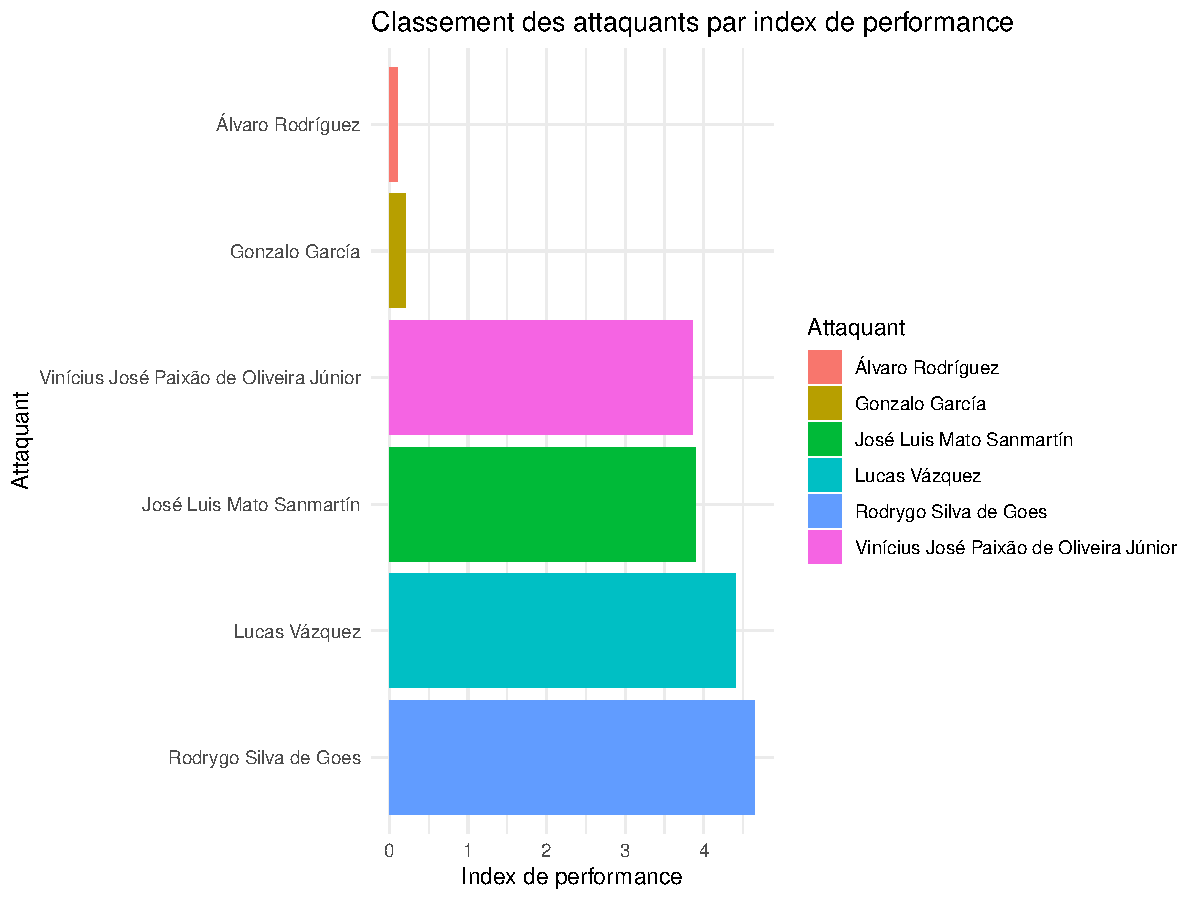
\includegraphics[width=0.8\linewidth]{Analyse_Impact_Performances_Joueurs_files/figure-latex/classeemnt-forwards-1} \end{center}

\subsubsection{Contributions des métriques à l'index de
performance}\label{contributions-des-muxe9triques-uxe0-lindex-de-performance}

Les buts marqués (goals) et les passes décisives (goal assists)
contribuent au graphique en termes de métriques principales, ainsi qu'à
l'index de performance des attaquants.

Le graphique met en évidence les rôles distincts des attaquants dans
l'équipe Certains, tels que Vinícius et Rodrygo, combinent leur habileté
à marquer et à créer des occasions, tandis que d'autres, tels que Lucas
Vázquez, se concentrent davantage sur un aspect spécifique.

Cette visualisation permet une meilleure compréhension des contributions
individuelles des joueurs et une optimisation de leur utilisation en
fonction de leurs forces respectives.

\begin{center}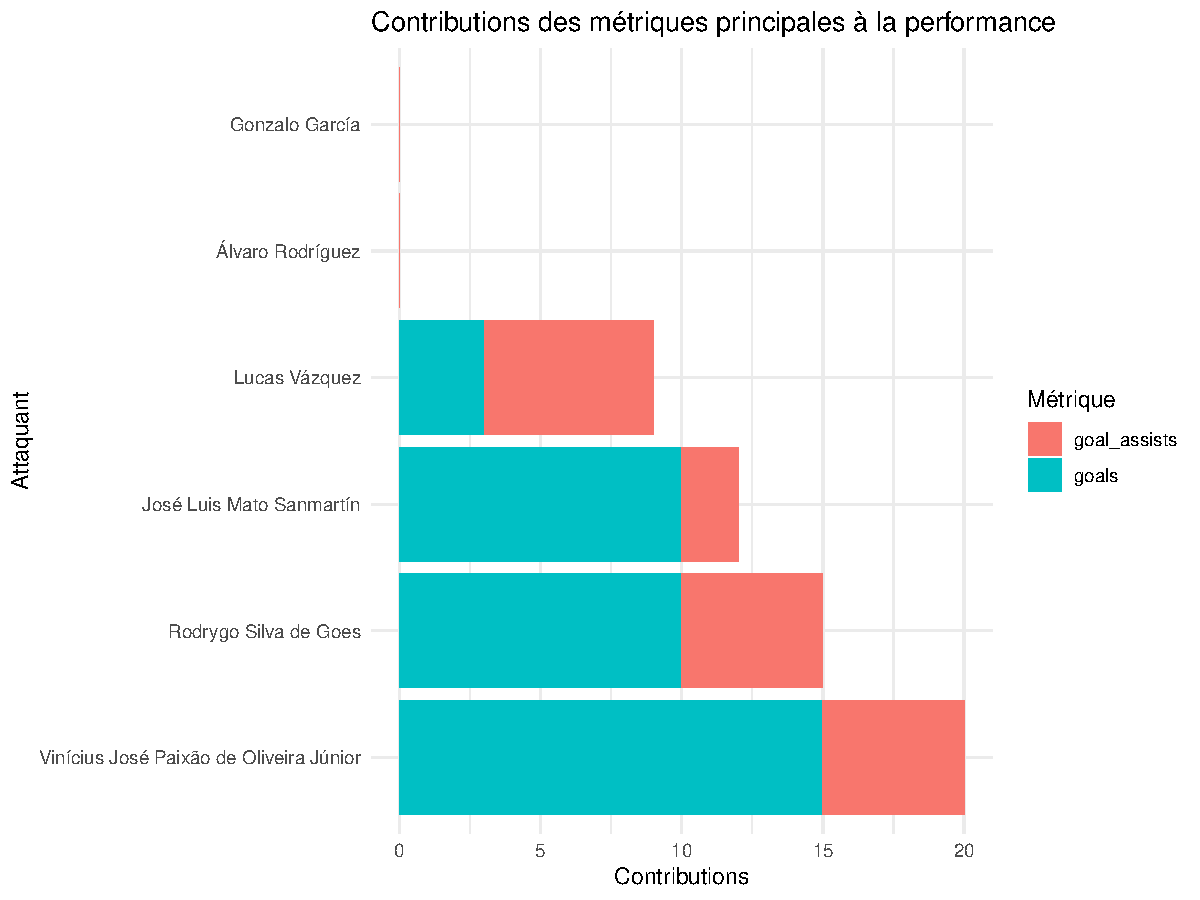
\includegraphics[width=0.8\linewidth]{Analyse_Impact_Performances_Joueurs_files/figure-latex/Contributions metrics-forwards-1} \end{center}

\subsubsection{Clustering des attaquants en fonction des
performances}\label{clustering-des-attaquants-en-fonction-des-performances}

\begin{center}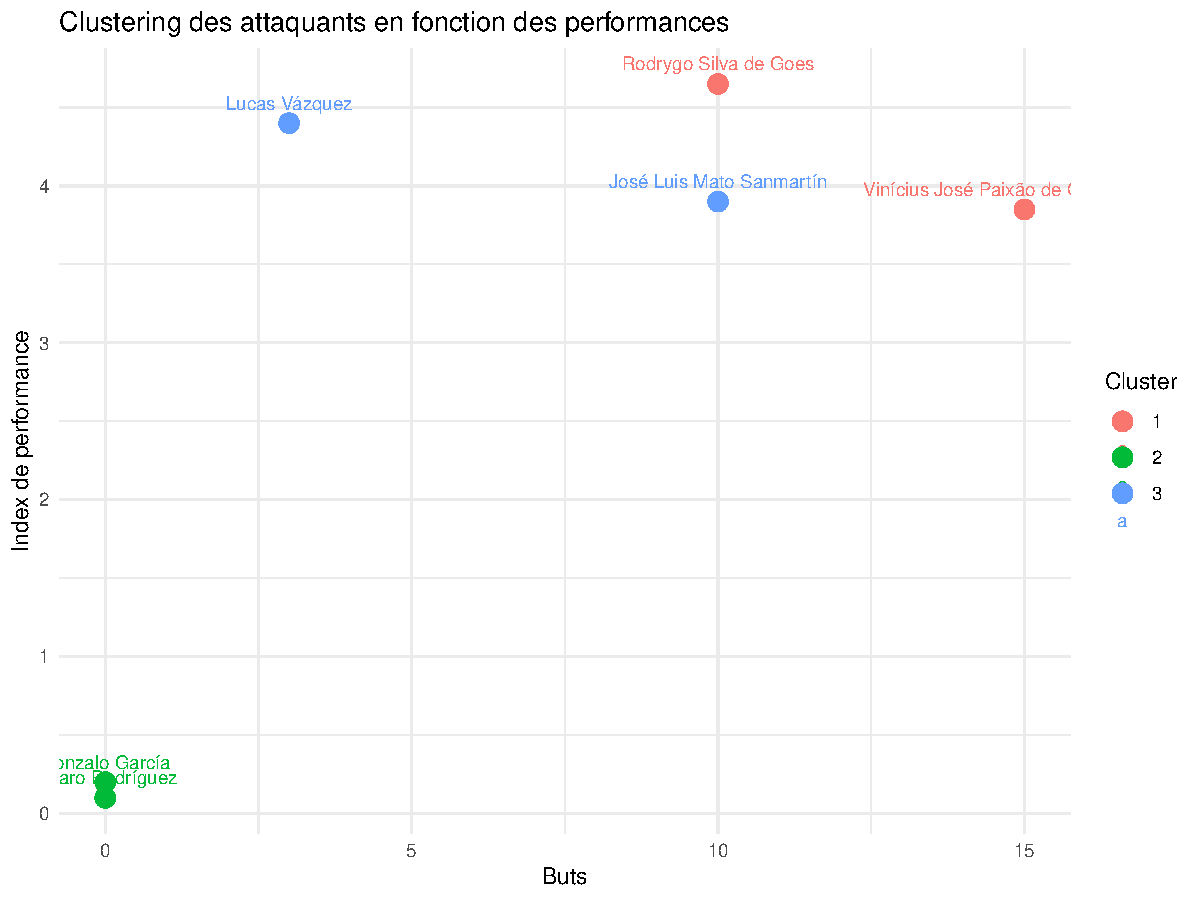
\includegraphics[width=0.8\linewidth]{Analyse_Impact_Performances_Joueurs_files/figure-latex/Clustering-forwards-1} \end{center}

\subsubsection{Calcul des corrélations entre performance index et les
metriques}\label{calcul-des-corruxe9lations-entre-performance-index-et-les-metriques}

\begin{center}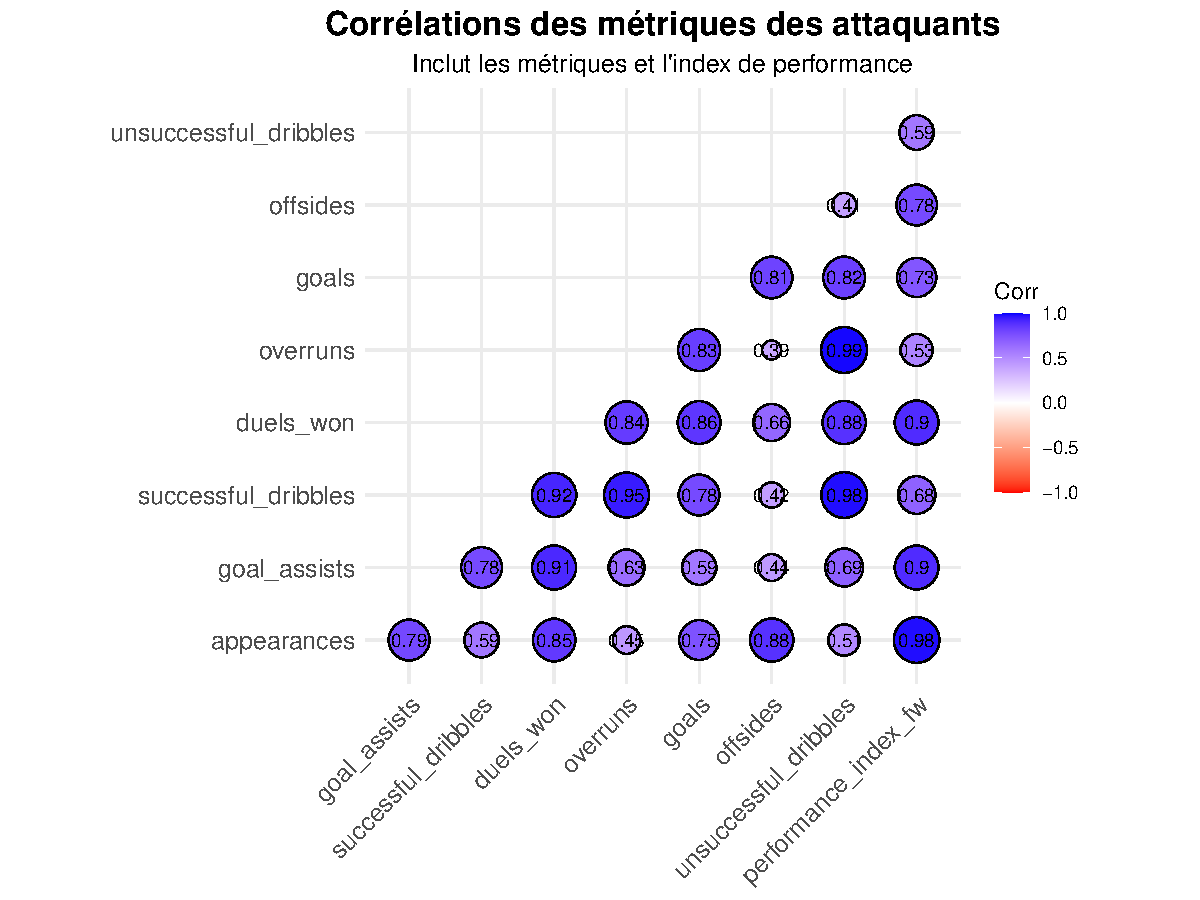
\includegraphics[width=0.8\linewidth]{Analyse_Impact_Performances_Joueurs_files/figure-latex/Correlation-forwards-1} \end{center}

\subsubsection{Répartition des contributions
offensives}\label{ruxe9partition-des-contributions-offensives}

Le diagramme en secteur représente la répartition des contributions
offensives pour chaque attaquant. Vinícius Júnior et Rodrygo se
partagent une large portion des contributions offensives, soulignant
leur rôle clé dans l'attaque.

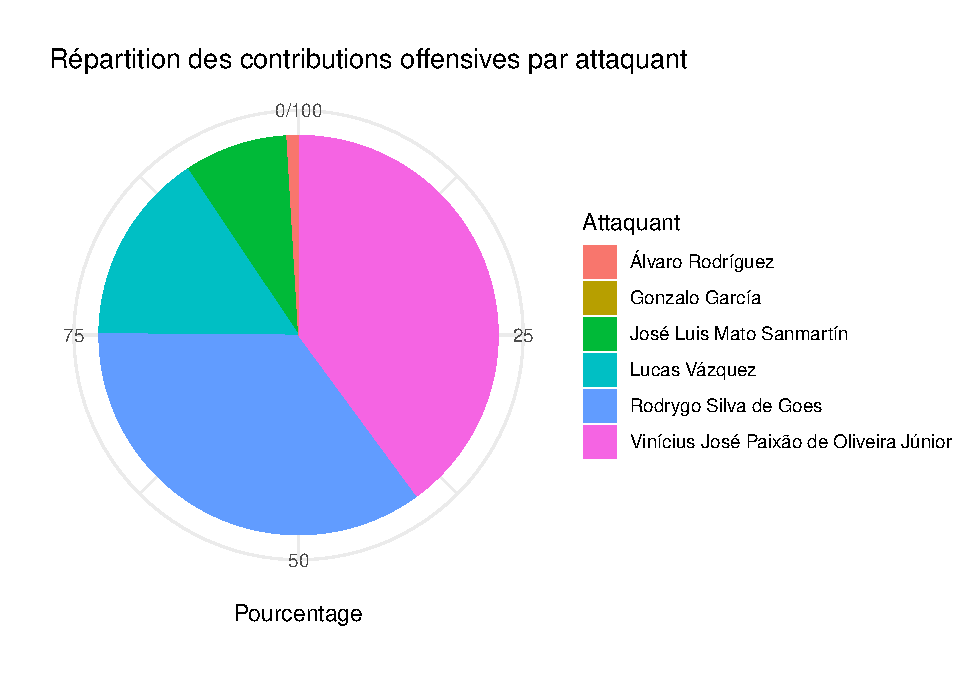
\includegraphics[width=0.8\linewidth]{Analyse_Impact_Performances_Joueurs_files/figure-latex/repartition-forwards-1}

\subsubsection{Analyse comparative : Efficacité des
tirs}\label{analyse-comparative-efficacituxe9-des-tirs}

Le graphique examine la relation entre les tirs cadrés et non cadrés en
fonction de l'index de performance des attaquants.

\begin{itemize}
\item
  On observe une corrélation positive : les joueurs qui effectuent plus
  de tirs cadrés ont également tendance à produire davantage de tirs non
  cadrés.
\item
  Les joueurs avec un index de performance élevé représentés par des
  couleurs proches du rouge combinent généralement un grand nombre de
  tirs cadrés et non cadrés. Cela reflète une activité offensive plus
  intense.
\end{itemize}

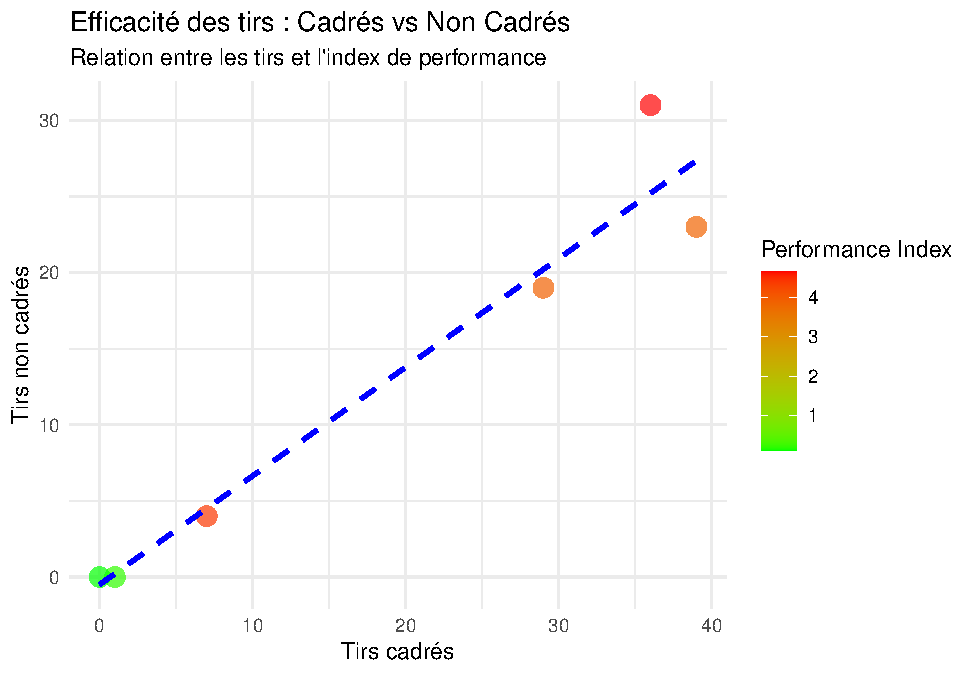
\includegraphics[width=0.8\linewidth]{Analyse_Impact_Performances_Joueurs_files/figure-latex/Cadrés vs Non Cadrés-forwards-1}

Ce graphique souligne que l'activité offensive, mesurée par le nombre de
tirs, joue un rôle crucial dans l'amélioration de l'index de
performance.

Cependant, il souligne également la nécessité d'améliorer la précision
des tirs, car une proportion élevée de tirs non cadrés peut réduire
l'efficacité globale des attaquants.

Ces informations peuvent être utilisées pour identifier les joueurs qui
nécessitent un entraînement spécifique afin d'optimiser leur impact dans
le jeu.

\section{Conclusion Générale et
Perspective}\label{conclusion-guxe9nuxe9rale-et-perspective}

En analysant les performances individuelles des joueurs, on a pu mettre
en évidence des points clés sur leur contribution respective.

Les métriques principales, telles que les buts marqués, les passes
décisives, et les actions défensives, ont révélé des rôles distincts et
des niveaux d'impact variés parmi les attaquants, les milieux de
terrain, les défenseurs et les gardiens.

Les joueurs comme Toni Kroos, Rodrygo Silva de Goes et Andrii Lunin ont
montré une grande constance et un impact significatif dans leurs zones
respectives du jeu.

Ces observations renforcent l'importance d'un suivi continu des
performances pour adapter les stratégies d'entraînement et de rotation.

Pour aller plus loin, il est essentiel d'effectuer une analyse
approfondie pour relier les performances individuelles à la performance
collective de l'équipe. Explorer cette relation est possible grâce au
dataset MatchesRM, qui est encore inexploité. Par exemple, il serait
pertinent d'évaluer :

\begin{itemize}
\item
  L'impact des performances individuelles sur les résultats des matchs :
  Comment les contributions clés influencent-elles les victoires, les
  défaites, ou les nuls ?
\item
  Les dynamiques collectives : Quels joueurs interagissent le mieux
  ensemble et comment les combinaisons spécifiques (attaquants et
  milieux, défenseurs et gardiens) influencent-elles la réussite de
  l'équipe ?
\item
  L'impact de l'audience sur les matchs et la relation entre les
  résultats et les matchs à domicile ou à l'extérieur.
\end{itemize}

En intégrant l'analyse des performances individuelles et des données des
matchs, il sera possible de mieux comprendre les liens entre les
statistiques et les résultats collectifs, cette approche permettra de
formuler des recommandations précises pour optimiser la stratégie
globale de l'équipe.

\end{document}
